\documentclass[a4paper]{article}

\usepackage{inputenc}
\usepackage[british,UKenglish]{babel}
\usepackage{amsmath}
%\usepackage{titlesec}
\usepackage{color}
\usepackage{graphicx}
\usepackage{fancyref}
\usepackage{hyperref}
\usepackage{float}
\usepackage{scrextend}
\usepackage{setspace}
\usepackage{xargs}
\usepackage{multicol}
\usepackage{nameref}

\usepackage{sectsty}
\usepackage{multicol}
\usepackage{multirow}
\usepackage[procnames]{listings}
\usepackage{appendix}
\usepackage{listings}

\newcommand\tab[1][1cm]{\hspace*{#1}}
\hypersetup{colorlinks=true, linkcolor=black}
\interfootnotelinepenalty=10000

\newcommand{\cleancode}[1]{\begin{addmargin}[3em]{3em}\texttt{\textcolor{cleanOrange}{#1}}\end{addmargin}}
\newcommand{\cleanstyle}[1]{\text{\textcolor{cleanOrange}{\texttt{#1}}}}


\usepackage[colorinlistoftodos,prependcaption,textsize=footnotesize]{todonotes}
\newcommandx{\commred}[2][1=]{\textcolor{Red}
{\todo[linecolor=red,backgroundcolor=red!25,bordercolor=red,#1]{#2}}}
\newcommandx{\commblue}[2][1=]{\textcolor{Blue}
{\todo[linecolor=blue,backgroundcolor=blue!25,bordercolor=blue,#1]{#2}}}
\newcommandx{\commgreen}[2][1=]{\textcolor{OliveGreen}{\todo[linecolor=OliveGreen,backgroundcolor=OliveGreen!25,bordercolor=OliveGreen,#1]{#2}}}
\newcommandx{\commpurp}[2][1=]{\textcolor{Plum}{\todo[linecolor=Plum,backgroundcolor=Plum!25,bordercolor=Plum,#1]{#2}}}

\def\code#1{{\tt #1}}

\def\note#1{\noindent{\bf [Note: #1]}}

\makeatletter
%% The "\@seccntformat" command is an auxiliary command
%% (see pp. 26f. of 'The LaTeX Companion,' 2nd. ed.)
\def\@seccntformat#1{\@ifundefined{#1@cntformat}%
   {\csname the#1\endcsname\quad}  % default
   {\csname #1@cntformat\endcsname}% enable individual control
}
\let\oldappendix\appendix %% save current definition of \appendix
\renewcommand\appendix{%
    \oldappendix
    \newcommand{\section@cntformat}{\appendixname~\thesection\quad}
}
\makeatother




\lstset{frame=, basicstyle={\footnotesize\ttfamily}}



\graphicspath{ {images/} }
\usepackage{ctex}
%-----------------------------------------BEGIN DOC----------------------------------------

\begin{document}
\renewcommand{\contentsname}{目\ 录}
\renewcommand{\appendixname}{附录}
\renewcommand{\appendixpagename}{附录}
\renewcommand{\refname}{参考文献} 
\renewcommand{\figurename}{图}
\renewcommand{\tablename}{表}
\renewcommand{\today}{\number\year 年 \number\month 月 \number\day 日}

\begin{titlepage}
    \begin{center}
        \vspace*{1cm}
 
        \Huge
        \textbf{Udacity机器学习工程师进阶纳米学位毕业项目报告}
 
        \vspace{0.5cm}
        \LARGE
        Rossmann Store Sales Prediction
 
        \vspace{1.5cm}
 
        \textbf{李懋}
 
        \vfill
 
        2018 Fall - 2019 Spring\\
        
 
        \vspace{0.8cm}
 
        %\includegraphics[width=0.4\textwidth]{university}
 
        \Large
        成都,中国\\
        2019年3月
 
    \end{center}
\end{titlepage}

%\title{{\Huge Udacity机器学习工程师进阶纳米学位毕业项目报告{\large\linebreak\\}}{\Large Rossmann Sales Prediction\linebreak}}
%please write your name, Student #, and Class # in Authors, student ID, and class # respectively
%\vspace{2cm}
%\textbf{姓 \ 名: 李懋}
%邮\ 箱:  772665912@qq.com\\
%手\ 机: 183-8021-4032\\\\
%CS 22014 流计算结构及其程序设计\\
%(2018 Fall - 2019 Spring)\\\\
%成都,中国\\

%\date{\today}
%\maketitle
%\newpage




%------------------------------------------TEXT--------------------------------------------

%----------------------------------------OVERVIEW-----------------------------------------

\section{问题定义} \label{overview}%------------------------------
\subsection{项目简介}
该项目是2018年秋季至2019年春季,优达学城  \href{https://www.udacity.com/}{Udacity} 机器学习工程师纳米学位毕业项目。题目本身来源于 2015 年的 Kaggle 比赛 \href{https://www.kaggle.com/c/rossmann-store-sales}{Rossmann Store Sales}. Rossmann 是来至于德国的的一家大型连锁药店,Rossmann 的经理希望能对各个门店未来六周的销售额进行预测,因为可靠的销售额预测能让经理提前进行合理的人力资源提前分配,从而提高资源的使用效率以及进行提前的备货等准备工作。门店的销售额会受很多因素的影响。

该项目的目标就是要基于 Rossmann 各个门店的信息(比如竞争者的距离、竞争者的存在时长,学校或者国家公共节假日、季节性和位置等)以及过往的销售情况来建模预测未来六周的销售额。项目使用到的数据集为 1115 个 Rossmann 门店的历史销售记录和这些门店的相关信息。项目需要最终的结果提交到 Kaggle 排行榜,排名为需要在public leader board 排进前 10\%,方可通过项目.
\subsection{问题称述}
项目要求预测的是门店未来六周的销售额,所以按照机器学习对问题的分类方法,很明显,预测的结果是连续数值,而不是离散值。因而,该项目属于回归 (Regression)问题,那么项目要完成的任务就是从所给的数据中提取出可能对销售额有影响的特征,建立有效的回归模型进行预测。具体来说,主要可以分为以下几步(其实也是所有机器学习问题应该遵循的流程 pipeline):
\begin{itemize}
    

\item{\textbf{数据探索}:通过探索性数据分析(Exploratory Data Analysis)来尝试了解数据的一些基本情况。主要需要应用到 Python 数据可视化分析,因为数据呈现更加直观。此外,像数据的分布情况、缺失情况等,可以通过 pandas 中的相关函数完成。做数据探索的目的是,对数据形成初始印象,为后面的特征工程(Feature Engineering)做准备和提供一些参考;}
\item{\textbf{数据预处理}:通过数据预处理(Pre-process the data)或者也可以叫 数据清洗 (Data Cleaning)过程来处理诸如类别信息、缺省值、时间序列信息等。也就是说,对于异常值 (outliners)需要做剔除等操作,对缺失值需要做补全 (fill-in) 等操作,这一步的目的是便于后续的特征提取;}
\item{\textbf{特征工程}:通过特征工程(Feature Engineering)来最大限度地提取出特征供后续的模型使用;特征在机器学习中就是指输入训练模型的变量,既可以是项目本身给定的原始数据中既有的,也可以通过原始数据来构造新的特征}
\item{\textbf{训练模型}:利用提取到的特征建立回归模型,在建模的过程中可以尝试通过特征选择和模型融合(feature selection and model ensemble)来争取达到比较好的预测效果。训练模型是在训练数据集上进行的,通常还可以将训练集分出一部分成为验证集 (Validation Data)}
\item{\textbf{预测结果}:具体到本个项目,最终期望达成的结果是,训练好的模型根据最后测试集(Test Data)中提供的门店的相关信息(比如促销,竞争对手信息等)和预测日当天以及前后一段时期的节假日等信息,能尽可能准确地对预测日的销售额进行预测。}

\end{itemize}
\subsection{计算平台资源}
机器学习模型训练,需要消耗大量的计算资源。即使是本项目,虽然数据量不算特别大,但是在个人电脑上训练也会遇到很多问题。因此,有必要对本项目中使用的计算资源平台做简要介绍,也方便对模型 performance 进行对比分析。

\begin{table}[htp]
\caption{计算平台配置}\label{tab:platform}
\begin{center}
	\begin{tabular}{|l|l|l|p{6cm}|}
	\hline
	\textbf{平台} & \textbf{CPU} & \textbf{Python 环境} & \textbf{GPU}\\ \hline \hline
	MBP 2017 Pro			& 8GB 	& Python 3 Anaconda	& 无\\ \hline
	Google Cloud  	& 30GB	&  Python 3 Anaconda	& 1 x NVIDIA Tesla P100
\\ \hline
	Google Colab	&  < 12GB & 不清楚 & 1 x NVIDIA Tesla K80 \\ \hline
	\hline
	\end{tabular}
\end{center}
\end{table}

本项目中,主要使用到了三个计算平台,其中 MBP 为 local machine,后二者为 Google 远程平台。最初,决定从 local machine 寻找新的云端平台,主要是有两个原因。首先,自己平时在上班,能够做本项目的时间很零碎,也不可能时时刻刻把笔记本带上,因而希望有一个远程平台,能够有空的时候都进行推进一下项目进度。其次,在项目进行到第二大部分,也就是决定探索 TPOT 框架模型的时候,发现本地的 8GB 计算资源完全不够用, kernel 不断 die,已经完全不能用了。

\begin{figure}[ht]
 \centering
 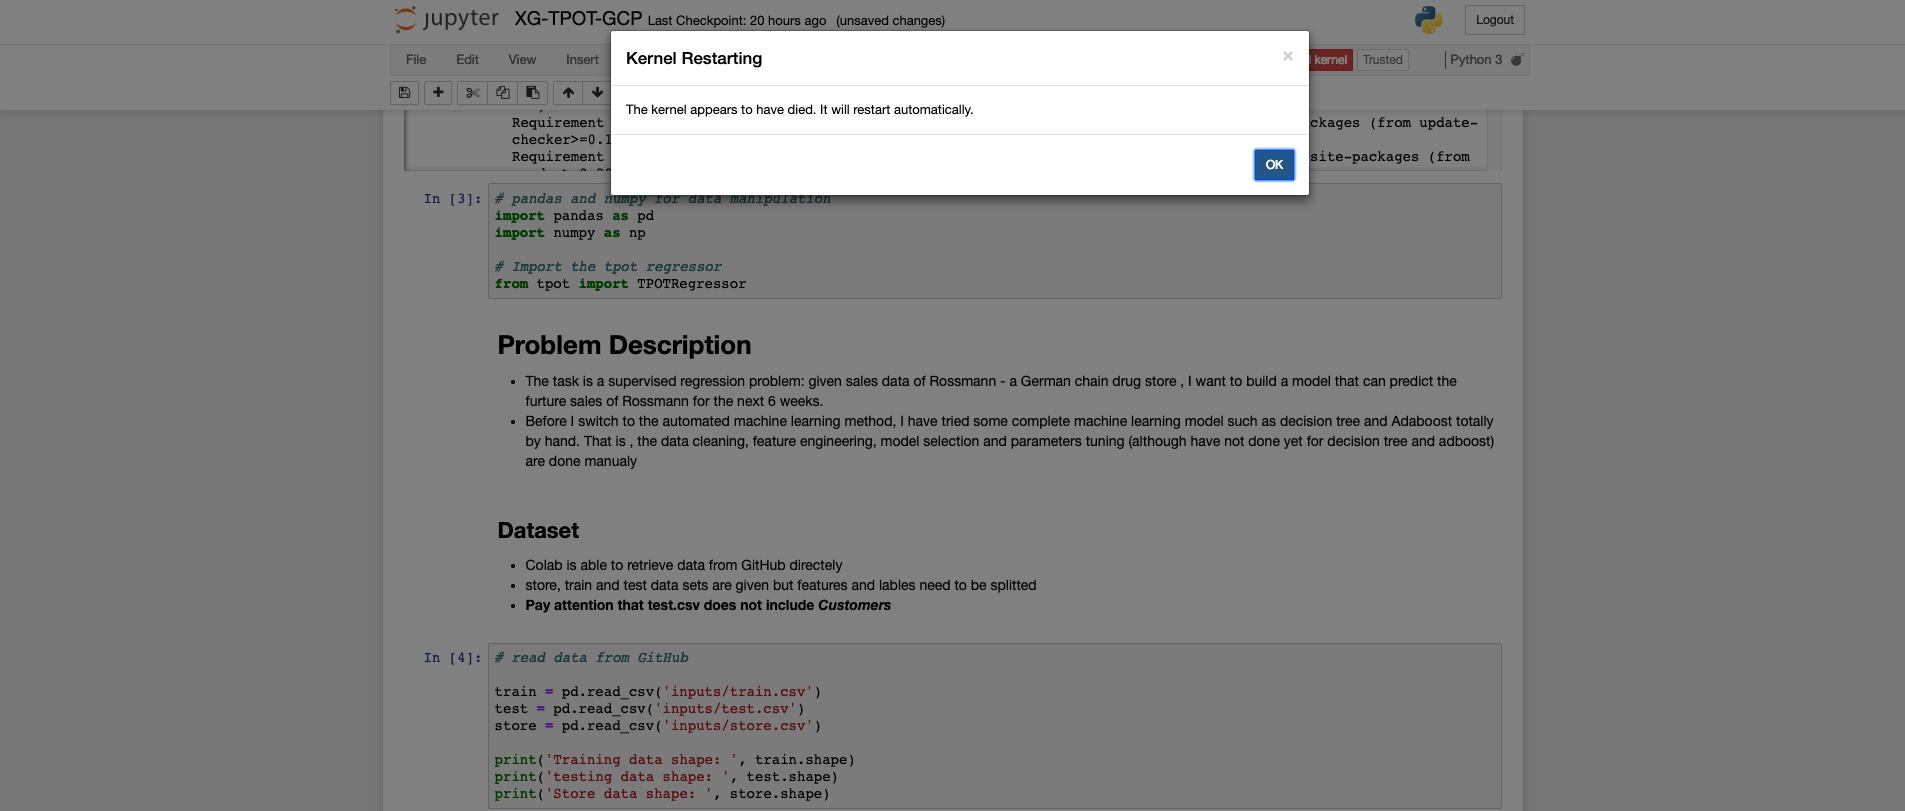
\includegraphics[height=5cm]{images/TPOT-kernel-die.png}
 \caption{TPOT 导致 Jupyter 崩溃}
 \label{fig:kernel-die}
\end{figure}

这个时候,通过搜索发现,谷歌的 colab 平台,不仅提供与 Google Drive 链接的云端存储,而且可以免费使用 GPU 资源。但是,实际试用之后,发现也不能满足要求,在其平台上也只能跑简单的模型。主要有以下原因:
\begin{itemize}


\item  RAM 严重不足。虽然 colab 名义上提供的 RAM 可以达到 13GB,实际上每次运算的时候,都是随机分配的,如图\ref{fig:colab}。不知道是因为处于国内网络环境使用代理的原因,还是其他什么未知原因,我最多的时候分配到的 RAM 都不超过 4G,显然还不如本地机。
\item 与 colab 的连接问题。既然 colab 是免费的环境,那么谷歌也相应对使用时间进行了限制。虽然,根据网上的资料,每个用户每天的最多连接时间可以有 12小时。但是,根据实际测试,一般一个小时左右就会报 connection timeout 错误。后来了解到,本来 colab 也不是为了长时间计算设计。

\end{itemize}
最后,综合以上因素,决定迁移到 Google Cloud 平台。即使,前期环境配置以及远程操作走了不少坑,后面还是还是值得的。

\begin{figure}[ht]
 \centering
 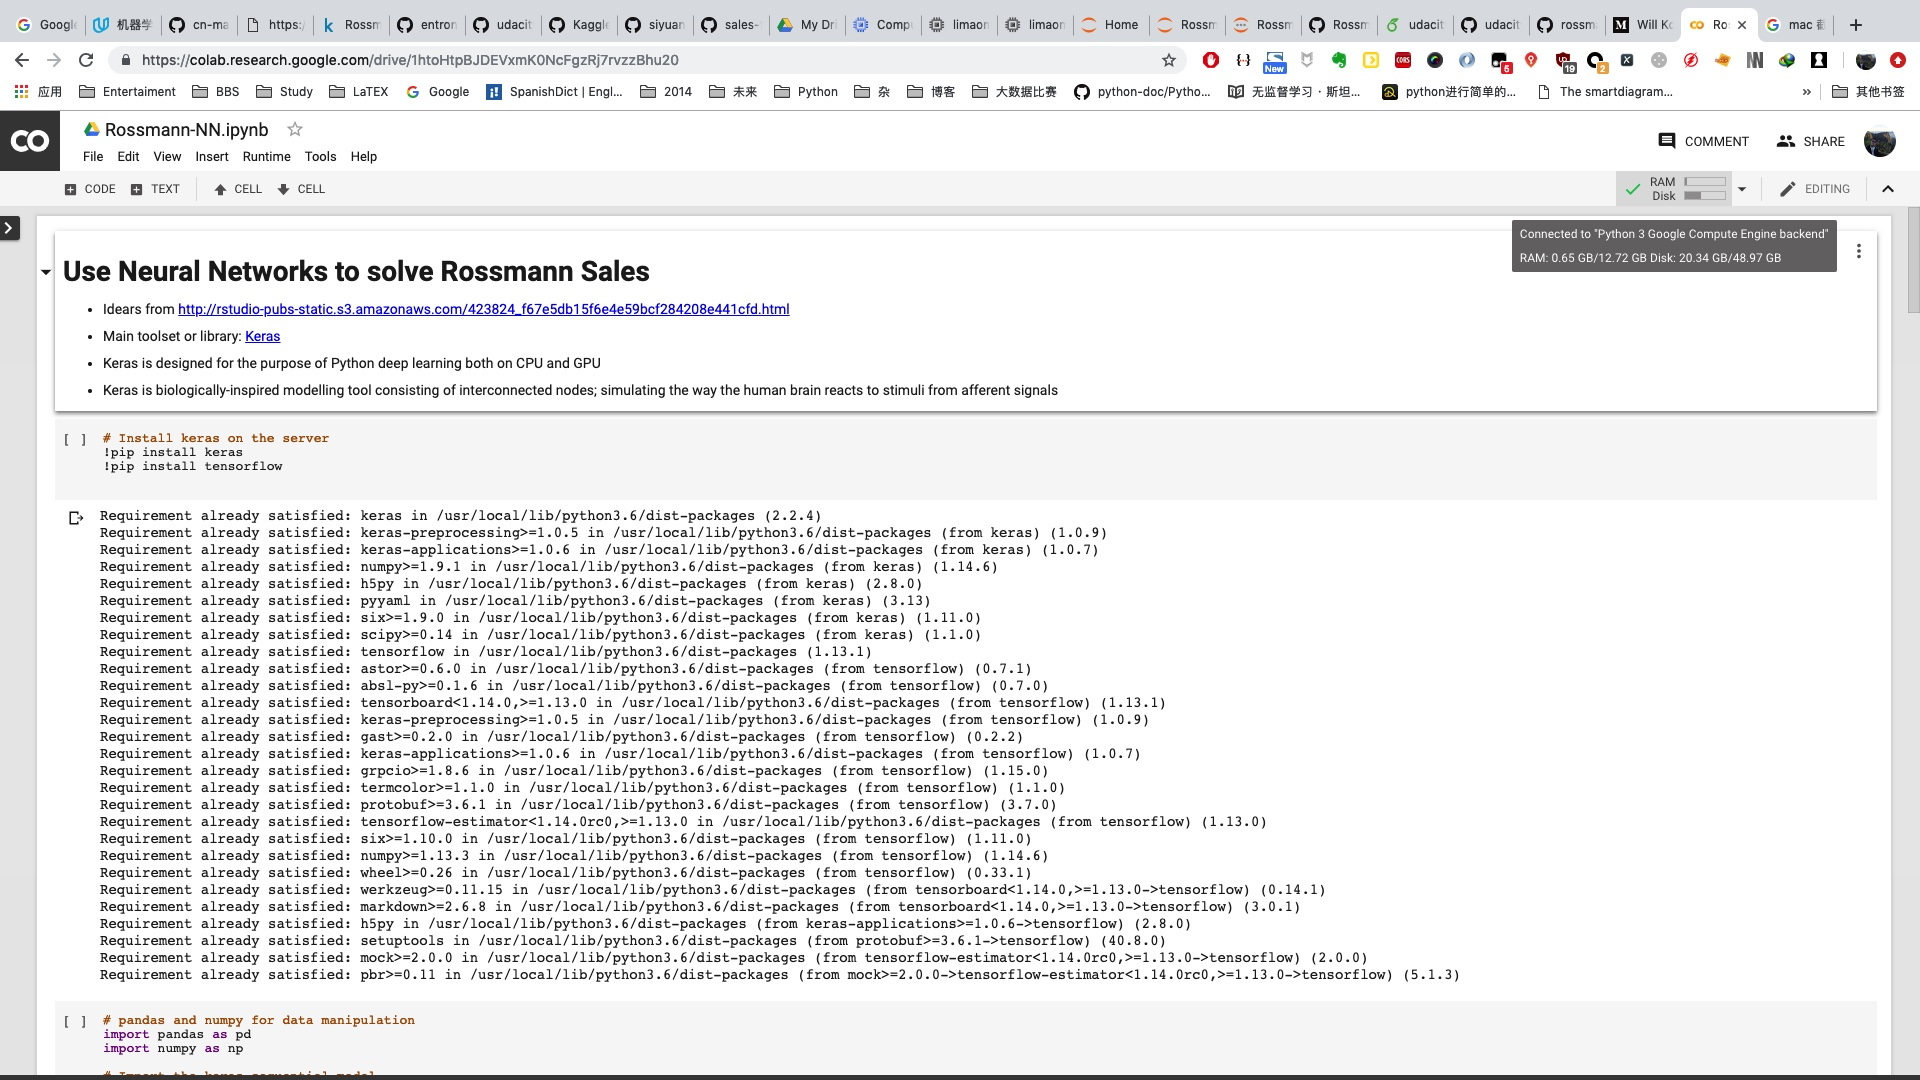
\includegraphics[height=5cm]{images/colab-ram.jpg}
 \caption{colab 平台 RAM 分配}
 \label{fig:colab}
\end{figure}

%------------------------------------Lab Process--------------------------------------

\newpage
%------------------------------
\section{数据探索分析 Data Exploration Analysis}\label{sub:eda}
\subsection{数据定义}
开始项目前,了解项目需要用的数据还是十分必要的。以下资料都来自 Kaggle \href{https://www.kaggle.com/c/rossmann-store-sales/data}{介绍}比赛介绍页面。项目提供的数据集中包含三个部分:train、test 和 store,train 数据集中包含了各个门店的历史销售额数据,store 数据集中包含了各个门店的一些补充信息,test 数据集被用于测试和评估模型。下面对各个数据集以及含义做一个详细介绍。
\begin{enumerate}
    \item train 数据集中一共包含 1017209 条数据记录,包含的数据含义如下:
    \begin{itemize}
        \item Store: 门店的数字标识
        \item DayOfWeek: 周一到周日的数字标识
        \item Date: 日期,从 2013-01-01 到 2015-07-31
        \item Sales: 单个门店在某个日期的销售额数据
        \item Customers: 单个门店在某个日期的顾客数
        \item Open: 指示门店是否开放(0 表示关闭,1 表示开放)
        \item Promo: 表示门店是否在进行促销(0 表示否,1 表示是)
        \item StateHoliday: 表示对应日期当天是否是法定假日(a 表示是公共假日,b 表示复活节,c 表示圣诞节,0 表示不是法定节日)
        \item SchoolHoliday: 表示对应日期当天是否是学校假日(0 表示不是,1 表示是)
    \end{itemize}
    \item store 数据集中一共包含 1115 条数据记录,包含的数据含义如下:
    \begin{itemize}
        \item Store: 门店的数字标识
        \item StoreType: 一共四种不同类型的门店(a,b,c,d)
        \item Assortment: 描述门店上架的商品类型(a 表示基本,b 表示额外,c 表示扩展)
        \item CompetitionDistance: 表示与最近的竞争对手门店的距离
        \item CompetitionOpenSinceMonth: 表示最近的竞争对手门店开业的月份
        \item CompetitionOpenSinceYear: 表示最近的竞争对手门店开业的年份
        \item Promo2: 表示一个门店是否进行了持续的促销(0 表示否,1 表示是)
        \item Promo2SinceWeek: 表示一个门店进行持续促销的开始的周数
        \item Promo2SinceYear: 表示一个门店进行持续促销的开始的年份
        \item PromoInterval: 表示门店开始促销的月份
    \end{itemize}
    \item test 数据集包含 41088 条数据记录,数据含义和 train 数据集一样:
    \begin{itemize}
        \item 没给销售额数据 'Sales' 和顾客数'Customers'
        \item 额外的 Id 用于 Kaggle 上数据的提交
    \end{itemize}

\end{enumerate}













\subsection{数据初探} \label{sub:da}
主要依靠 Pandas 和 Numpy 对 train, store, test 数据集进行探索性分析。同时,还要发现异常值,以及处理空缺值。本小节,所有 figure 以及源代码都可以在 \href{https://github.com/lidatou1991/udacity_final_rossmann/blob/master/rossmann_final_EDA.ipynb}{这里找到}。
\subsubsection{train 数据集探索}
train 数据集记录的是之前一段时间的销售情况,其中最重要的就是顾客数以及销售量。使用 plt 绘出其分布如下:

\begin{figure}[ht]
 \centering
 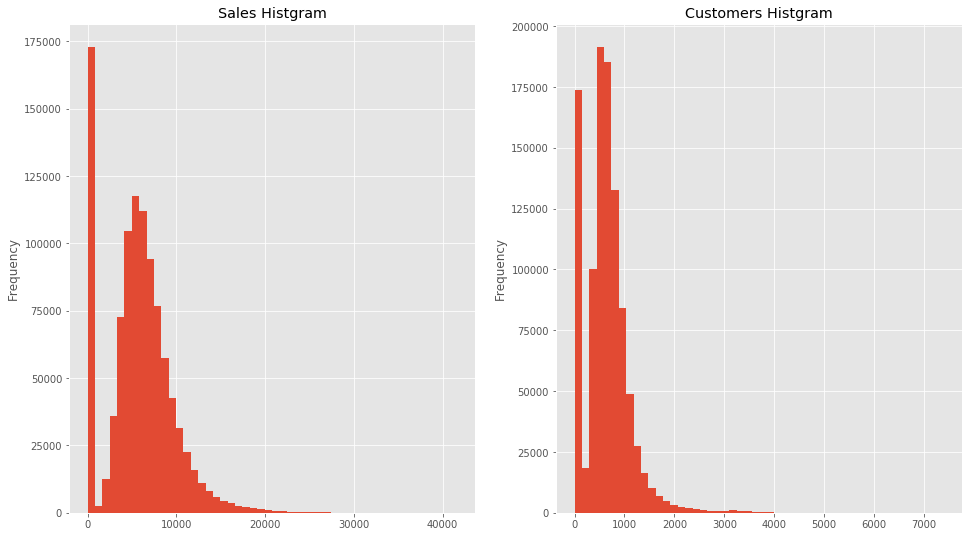
\includegraphics[height=5cm, width=0.95\textwidth]{images/train-hist.png}
 \caption{Sales 以及 Customers 直方图分布}
 \label{fig:train-hist}
\end{figure}
从上图中,可以看到,训练数据中包含很多 sales = 0 的数据。也就是说,商店的销量为0. 这些数据要么是因为商店没有开门,或者可能是记录错误等造成的异常。用这种数据来训练模型,是没有意义的,因而首先把这类 sales = 0 的数据删除。

然后,来看销量是否与当天是星期几,也就是 DayOfWeek 有关。考察销量在一周的每天的平均值分布。非常明显的一个变化发生在 DayOfWeek =7,也就是星期天。如果没有除了训练集中销量等于0的数据,可以看到星期天的平均销量是很低的,这是因为很多商店在星期天都关门,必然导致很多商店在星期天销量都是0。因而,这种情况下也就拉低了所有商店在星期天的平均销量。但是,如果删除了销量为0的数据,那么可以看到星期天的平均销量不算低,甚至还是比较高的。这是因为,其实删掉的 Sales = 0的数据,都是星期天关门的商店的数据。也就是,剩下来的数据都是星期天开门的商店数据。可以看到,只要商店星期天是开门的,销量并不差。但是,这两种情况下,都可以明显看到\textbf{每天的销量和当天是星期几关系还是很大的,才会导致每天平均销量有波动}。


因此,在预测数据的时候,十分有必要考虑当天是星期几。也就是说,DayOfWeek 这个特征。甚至于,在后面还分析了单一商店在一周的每天销量的平均分布,将其作为新的 feature 加入到训练数据中。
\begin{figure}[ht]
 \centering
 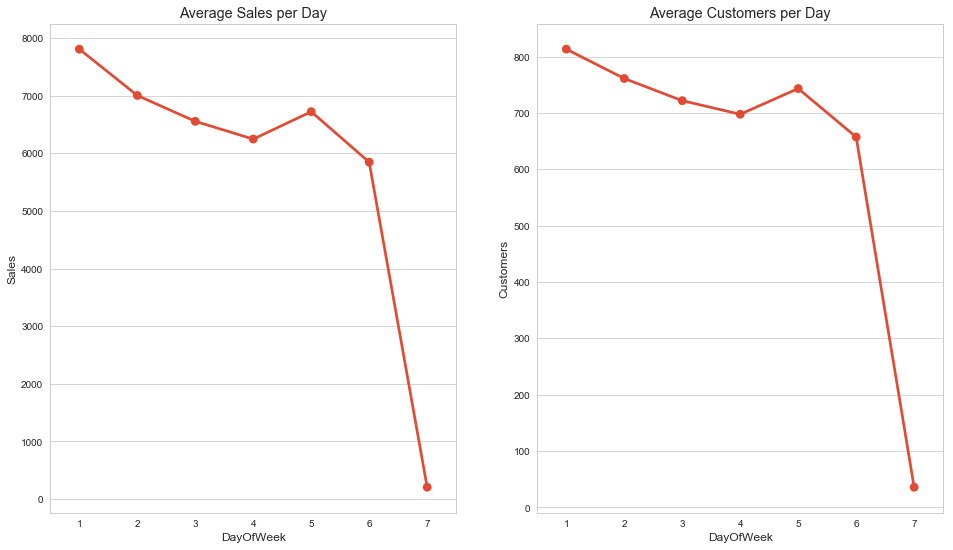
\includegraphics[height=5cm]{images/train-perday-nofilter.png}
 \caption{未删除 Sales=0 情况下每天的平均销量}
 \label{fig:nofilter}
\end{figure}

\begin{figure}[ht]
 \centering
 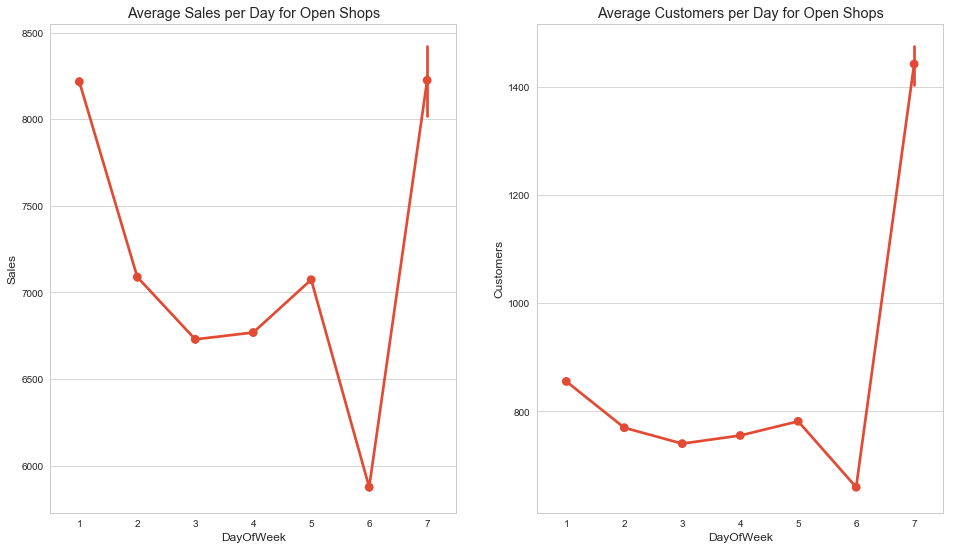
\includegraphics[height=5cm]{images/train-per-day-filter.png}
 \caption{删除 Sales=0 情况下每天的平均销量}
 \label{fig:filter}
\end{figure}

再看销量与月份的关系。可以看到销量与月份之间,存在周期关系,在每年的10-12月,销量会有比较大的提升。但是,其他时间段,每月的平均销量还是大致稳定的,相对平滑,没有明显的突变。我们需要预测的时间段,并不属于10-12月。而且,时间也只有6周,不到两个月,相对月均的销量还是稳定的。从分年度的销量随月份变化图上,也可以看到相同规律。因此,可以先暂时不考虑销量与月份之间的关系。
\begin{figure}[ht]
 \centering
 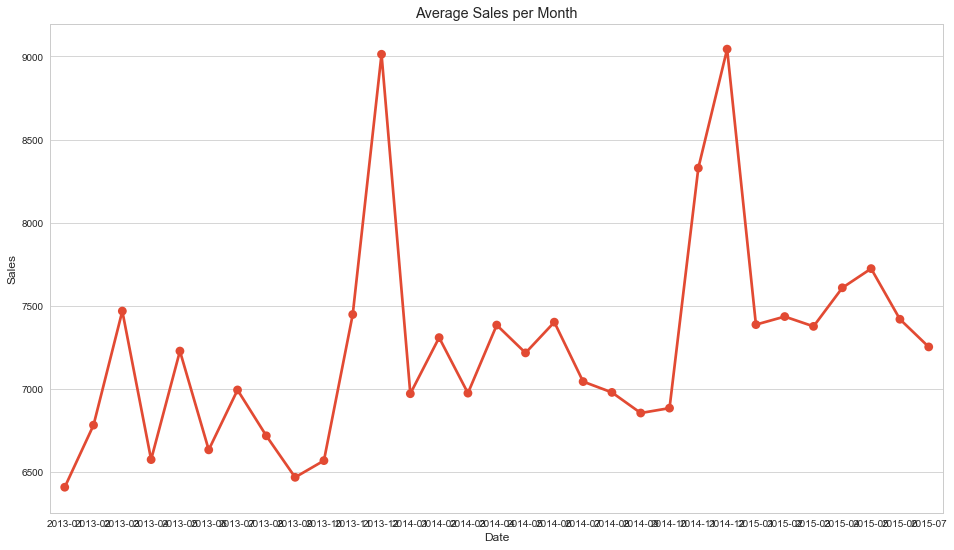
\includegraphics[height=5cm]{images/sales-month.png}
 \caption{平均每月销量}
 \label{fig:month}
\end{figure}

\begin{figure}[ht]
 \centering
 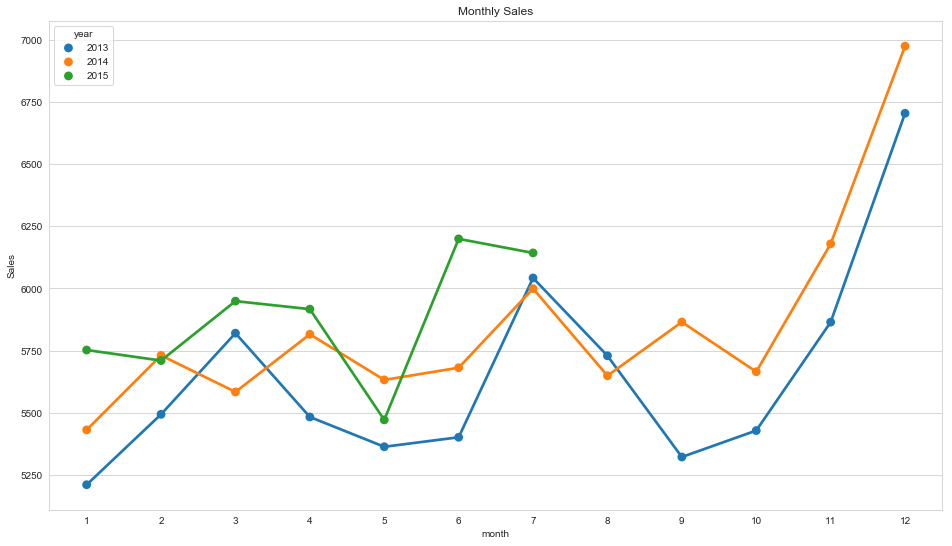
\includegraphics[height=5cm]{images/month-sale-by-year.png}
 \caption{分年度平均每月销量}
 \label{fig:month-by-year}
\end{figure}

我们可以看到,平均到每个月,所有商店的销量的平均值是存在波动的。而且,分年度来看,即使是相同的趋势,不同年度在相同月份的销量平均值也是不同的。因此,在这里至少我们可以确定两个对销量有影响的特征:年度 (year) 和月份 (month)。

那么,我们自然而然想到,在某一个月之中,平均到每天的销量会不会有某种波动呢。我们分别选取三年期间训练数据,在二月份每天的平均销量,以及分年度的数据来观察。图\ref{fig:feb} 可以看做是图\ref{fig:feb-by-year}的三条曲线的平均求和。通过图像,我们可以明确一点,甚至于需要预测的当天在一个月中是哪一天,都是可以作为预测模型的特征的。

\begin{figure}[ht]
 \centering
 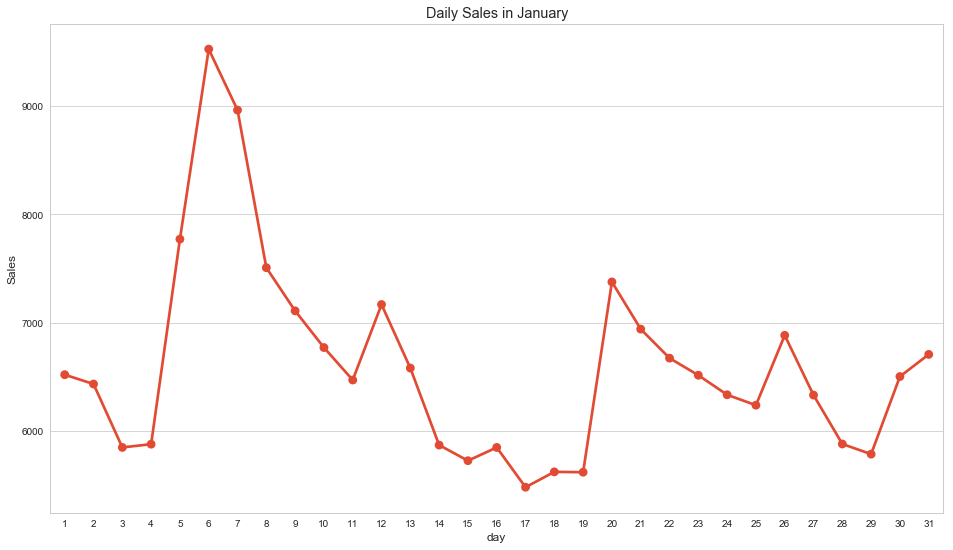
\includegraphics[height=5cm]{images/daily-in-month.png}
 \caption{2月平均每天销量}
 \label{fig:feb}
\end{figure}

\begin{figure}[ht]
 \centering
 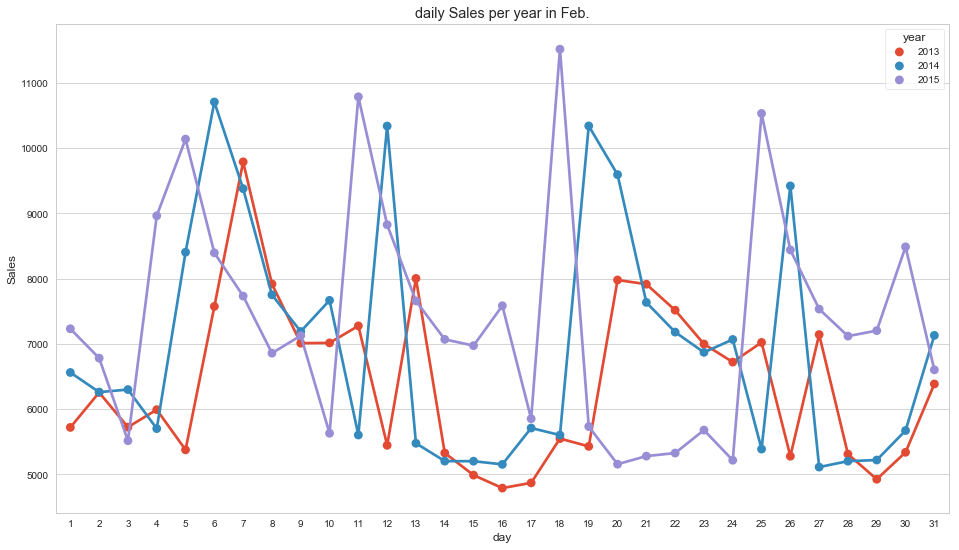
\includegraphics[height=5cm]{images/feb-daily-sale.png}
 \caption{分年度2月平均每天销量}
 \label{fig:feb-by-year}
\end{figure}



至于说 train 数据集中,整个时间段销量对每天的变化。从图中我实在看不出什么规律。可能和long term/ short term memory 这一类细分的问题相关。但是由于项目时间所限制,实在没时间再往下细细研究。因为,其实本项目从本质上来看,还可以看为连续时间序列的预测问题。和股票等预测有关,自己只是隐约有印象。我决定还是首先专注于之前项目中用到过的经典的机器学习模型。

\begin{figure}[ht]
 \centering
 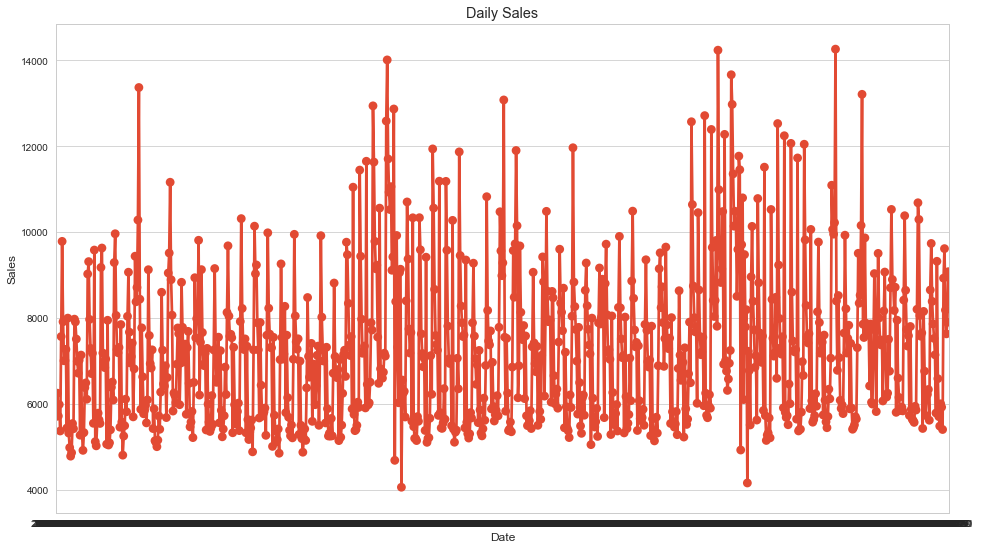
\includegraphics[height=5cm]{images/sale-daily.png}
 \caption{每天的销量变化}
 \label{fig:daily}
\end{figure}

\subsubsection{假期/商店类型/促销等对销量的影响}

在 train 数据集中,还有几个 categorical features 对销量可能有影响,值得探究。
\begin{itemize}

\item 假期的影响。不同假期对销量有一定影响,因此这个 feature 也予以保留。但是,确实暂时不能继续深挖出 deep feature 或者构造新的 feature添加到训练数据中。

\begin{figure}[ht]
 \centering
 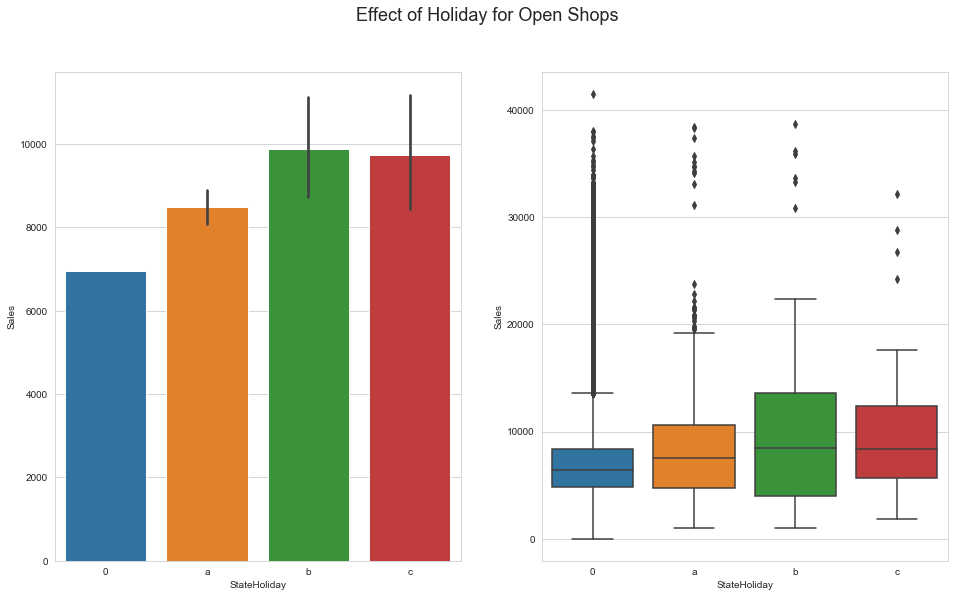
\includegraphics[height=5cm]{images/effect-holiday.png}
 \caption{每假期对销量的影响}
 \label{fig:holiday}
\end{figure}

\item 药店类型的影响。从图中,可以很明显看到,storetype 和 assortment 都为 b 的药店,不管是顾客数量,还是销量,都明显高于其他类型。因而,这两个 categorical feature 都需要保留。

\begin{figure}[ht]
 \centering
 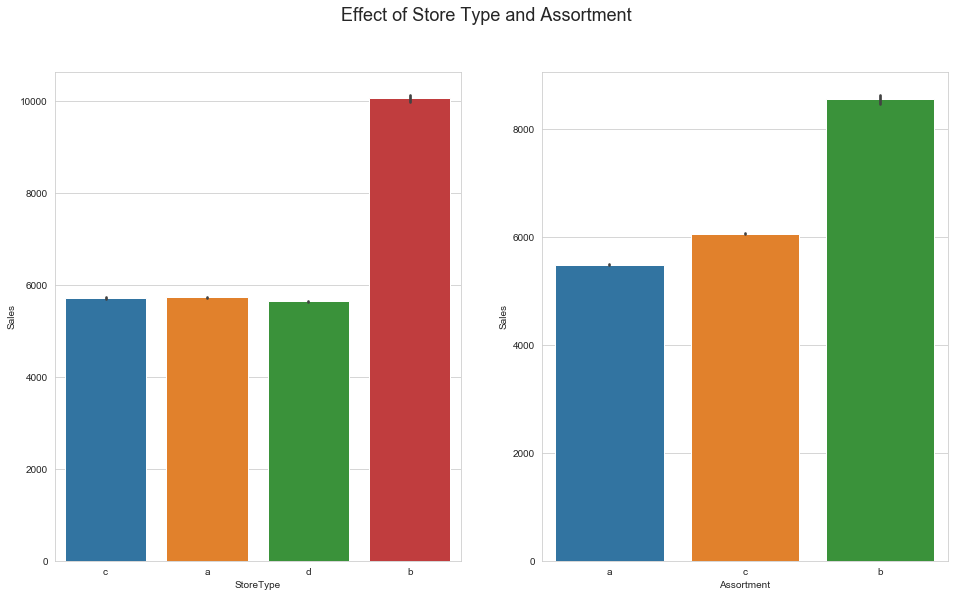
\includegraphics[height=5cm]{images/store-type.png}
 \caption{商店类型对销量的影响}
 \label{fig:storetype}
\end{figure}

\item 促销活动的影响。从常理上讲,促销活动肯定对销量是有影响的。但是,药店不同于百货公司等,顾客是否会单纯为了促销活动就去增加采购药品,这一点我还是存在疑虑的。从图上可以看到,促销活动确实也起到了一定的拉动销量的作用。因而,这一 feature 予以保留。但是,就没有构造新增 feature.
\begin{figure}[ht]
 \centering
 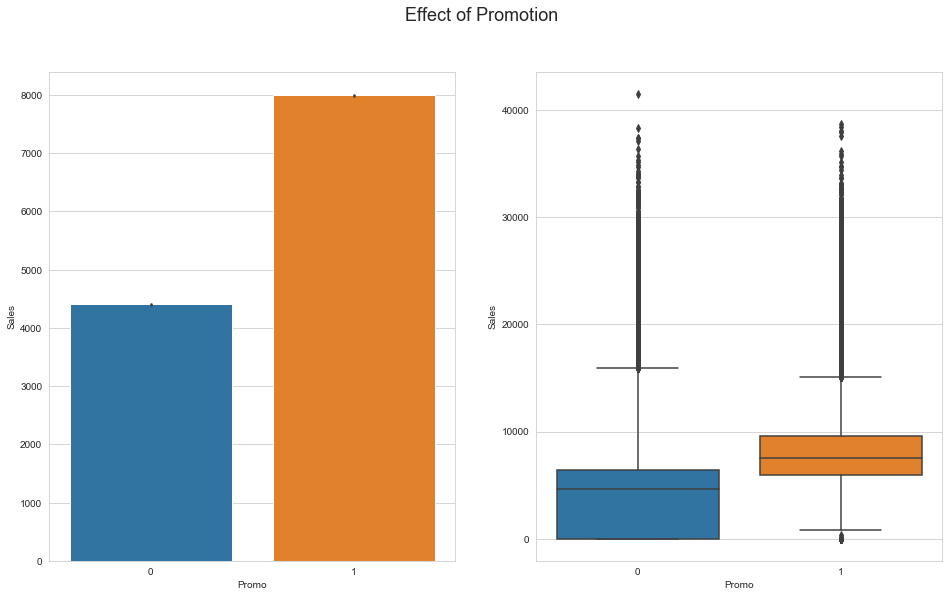
\includegraphics[height=5cm]{images/effect-promo.png}
 \caption{促销活动对销量的影响}
 \label{fig:promo}
\end{figure}
\end{itemize}



\subsubsection{竞争者对销量的影响}
这一点拿出来单独讲,是因为在看到结果图之前,实际结果与自己的分析是完全相反的。从图中可以看到,同一个销量下,竞争者距离越近,达到该销量的商店数量越多。也就是对单个商店来说,竞争者越近,其达到更高销量的几率更好。与之前自己认为的,竞争者可能削减销量完全相反。一种合理的解释是,竞争者越多,商圈氛围更浓厚,人流量也越大,因而销量可以增长。不管怎样,这么看来这一 feature 也是需要保留的。
\begin{figure}[ht]
 \centering
 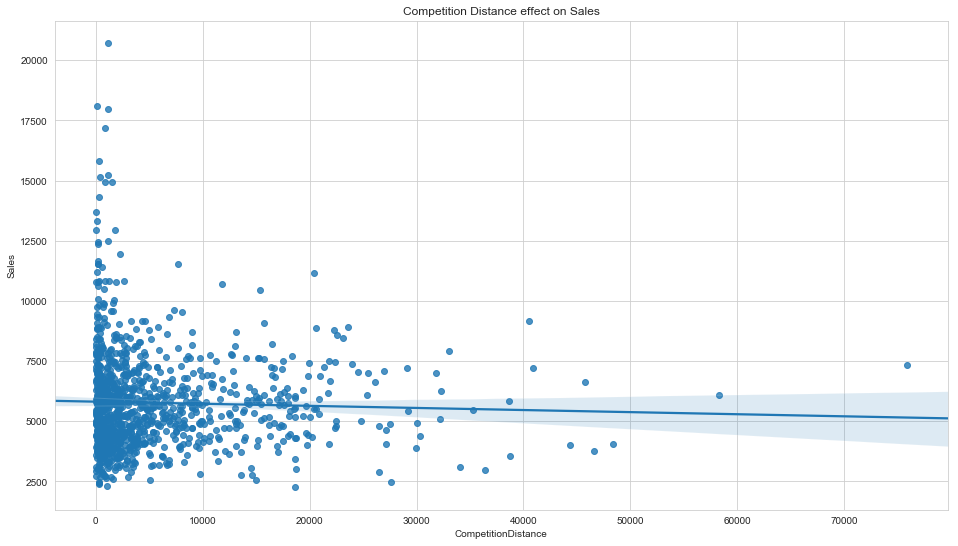
\includegraphics[height=5cm]{images/comp-distance.png}
 \caption{竞争者存在远近对销量的影响}
 \label{fig:distance}
\end{figure}


\subsubsection{顾客数量对销量的影响}
显而易见,顾客数代表了人气,商店的销量一定是和一天到访的顾客数量的多少息息相关的。那么,二者之间的关系可以从图\ref{fig:customres}看出:高度的正相关性。但是,尤其需要注意的是,在 test 数据集中,并不包括顾客数量 Customers 这一特征的。这是因为,很明显,要预测未来某一天顾客的数量,和本身项目的目标:预测未来某一天的销量,几乎是同等难度的问题。那么,如何将顾客数量这一特征考虑到模型中呢?

在\href{https://solgirouard.github.io/Rossmann_CS109A/notebooks/feature_engineering.html}{这篇文章}中,作者将 Customers 这一特征构造出的新特征,称为 Proxy Feature (代理特征)。也就是说,通过一系列变换、转化,将 Customers 融入到其他新造的特征中。虽然很多 GitHub 方案都做了这个步骤,但是还没有专门提出代理特征这一概念的。

在后面的特征工程中,会讲解如何构造单一商店平均顾客数等新特征,来融入 Customers 这一重要,但是又在 test 数据集中没有的特征的。

图\ref{fig:matrix}的是训练数据集中,各个特征与销量的相关性数矩阵。颜色越浅,代表正相关性越高,我们可以看到 open与 sales 呈现出最高的相关性,这个很容易理解,如果 open = 0,那么商店的销量一定是为零的。
\begin{figure}[ht]
 \centering
 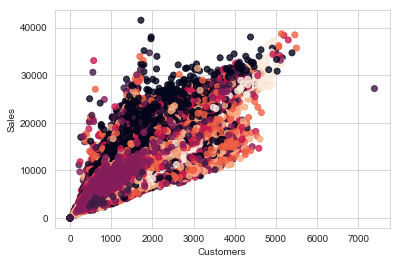
\includegraphics[height=6cm]{images/customers.png}
 \caption{顾客数量对销量的影响}
 \label{fig:customres}
\end{figure}

\begin{figure}[ht]
 \centering
 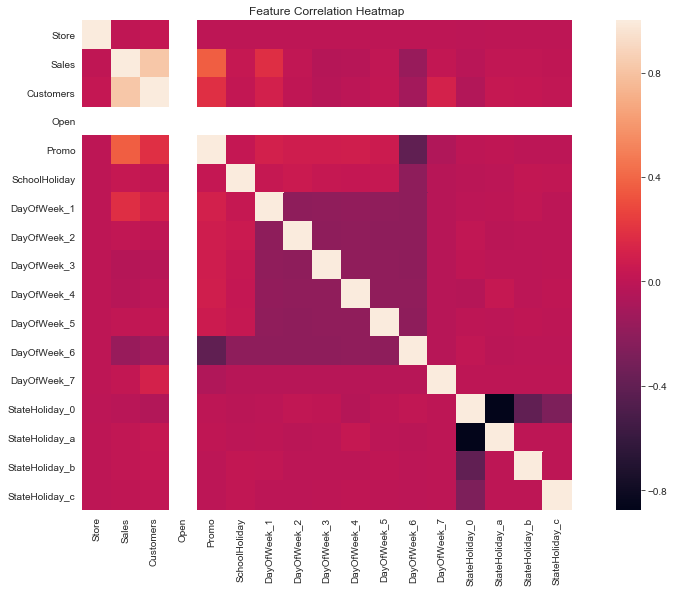
\includegraphics[height=5cm]{images/corr-heatmap}
 \caption{相关系数矩阵热力图}
 \label{fig:matrix}
\end{figure}

%\subsection{实验结果和分析}\label{sub:ptxeva}
%请在这一节详细说明需要分析的内容。
% --------------------------------Evaluation----------------------------------------
\section{特征工程 Feature Engineering}\label{fe}
\subsection{数据清洗} \label{sub:clean}\
\subsection{自动化特征工程}
使用的是自动化根据 featuretools,参考了\href{https://github.com/WillKoehrsen/automated-feature-engineering/blob/master/walk_through/Automated_Feature_Engineering.ipynb}{文章},由于内容实在太多,在这里就不在赘述。详细的介绍,都在 notebook 中。
\subsection{决策树模型} \label{sub:dt}
对应的 notebook 地址\href{https://github.com/lidatou1991/udacity_final_rossmann/blob/master/DT-model.ipynb}{在这里}
\subsection{Adaboost 模型} \label{sub:adboost}
对应的 notebook 地址 \href{https://github.com/lidatou1991/udacity_final_rossmann/blob/master/Adaboost.ipynb}{在这里}
\section{自动机器学习 Automated Machine Learning}\label{tpot}
机器学习流水线包括以下几个步骤:
\begin{itemize}
    \item 特征预处理: 填充缺失值,缩放,构建新的特征
    \item 特征选择: 降维
    \item 模型选择: 对多个模型进行评估
    \item 调参: 找到最佳的模型超参数设置
\end{itemize}
对以上的四个步骤进行组合你可以得到几乎无限多种流水线,而每个问题的最佳解决方式都不一样。设计一个机器学习流水线是一个非常消耗时间以及容易踩坑的过程,所以我们一般无法遍历所有流水线,也就是说你永远不知道你设计出来的流水线是不是最优的。这个时候,机器学习自动化出现了,它可以帮助你评估成千上万种可能的流水线的表现,自动找出最优的(或接近最优的)解决方案。

TPOT 是一种基于遗传算法优化机器学习管道(pipeline)的 Python 自动机器学习工具。遗传算法对于建立机器学习模型的主要好处就是深度的探索。对于人来说,即使没有时间的限制,也无法尝试完所有的预处理、模型、超参数的组合,毕竟个人的知识和想象力是有限的。而遗传算法对于任何机器学习流水线都不会有初始的偏见(人类可能会根据自己的经验,产生一些偏见),每一条流水线都会被客观地评估。此外,遗传算法中的适应度函数使得流水线探索空间中,最有潜力的组合区域比表现差的区域探索地更为彻底,这也是遗传算法的一大优势。简单来说,就是 TPOT 可以智能地探索数千个可能的 pipeline,为数据集找到最好的 pipeline,从而实现机器学习中最乏味的部分。

从下图\ref{tpot}中我们可以看到,TPOT 可以自动地完成特征工作(特征选择,特征预处理,特征构建等),同时也可以进行模型的选择和参数的调优。

\begin{figure}[ht]
 \centering
 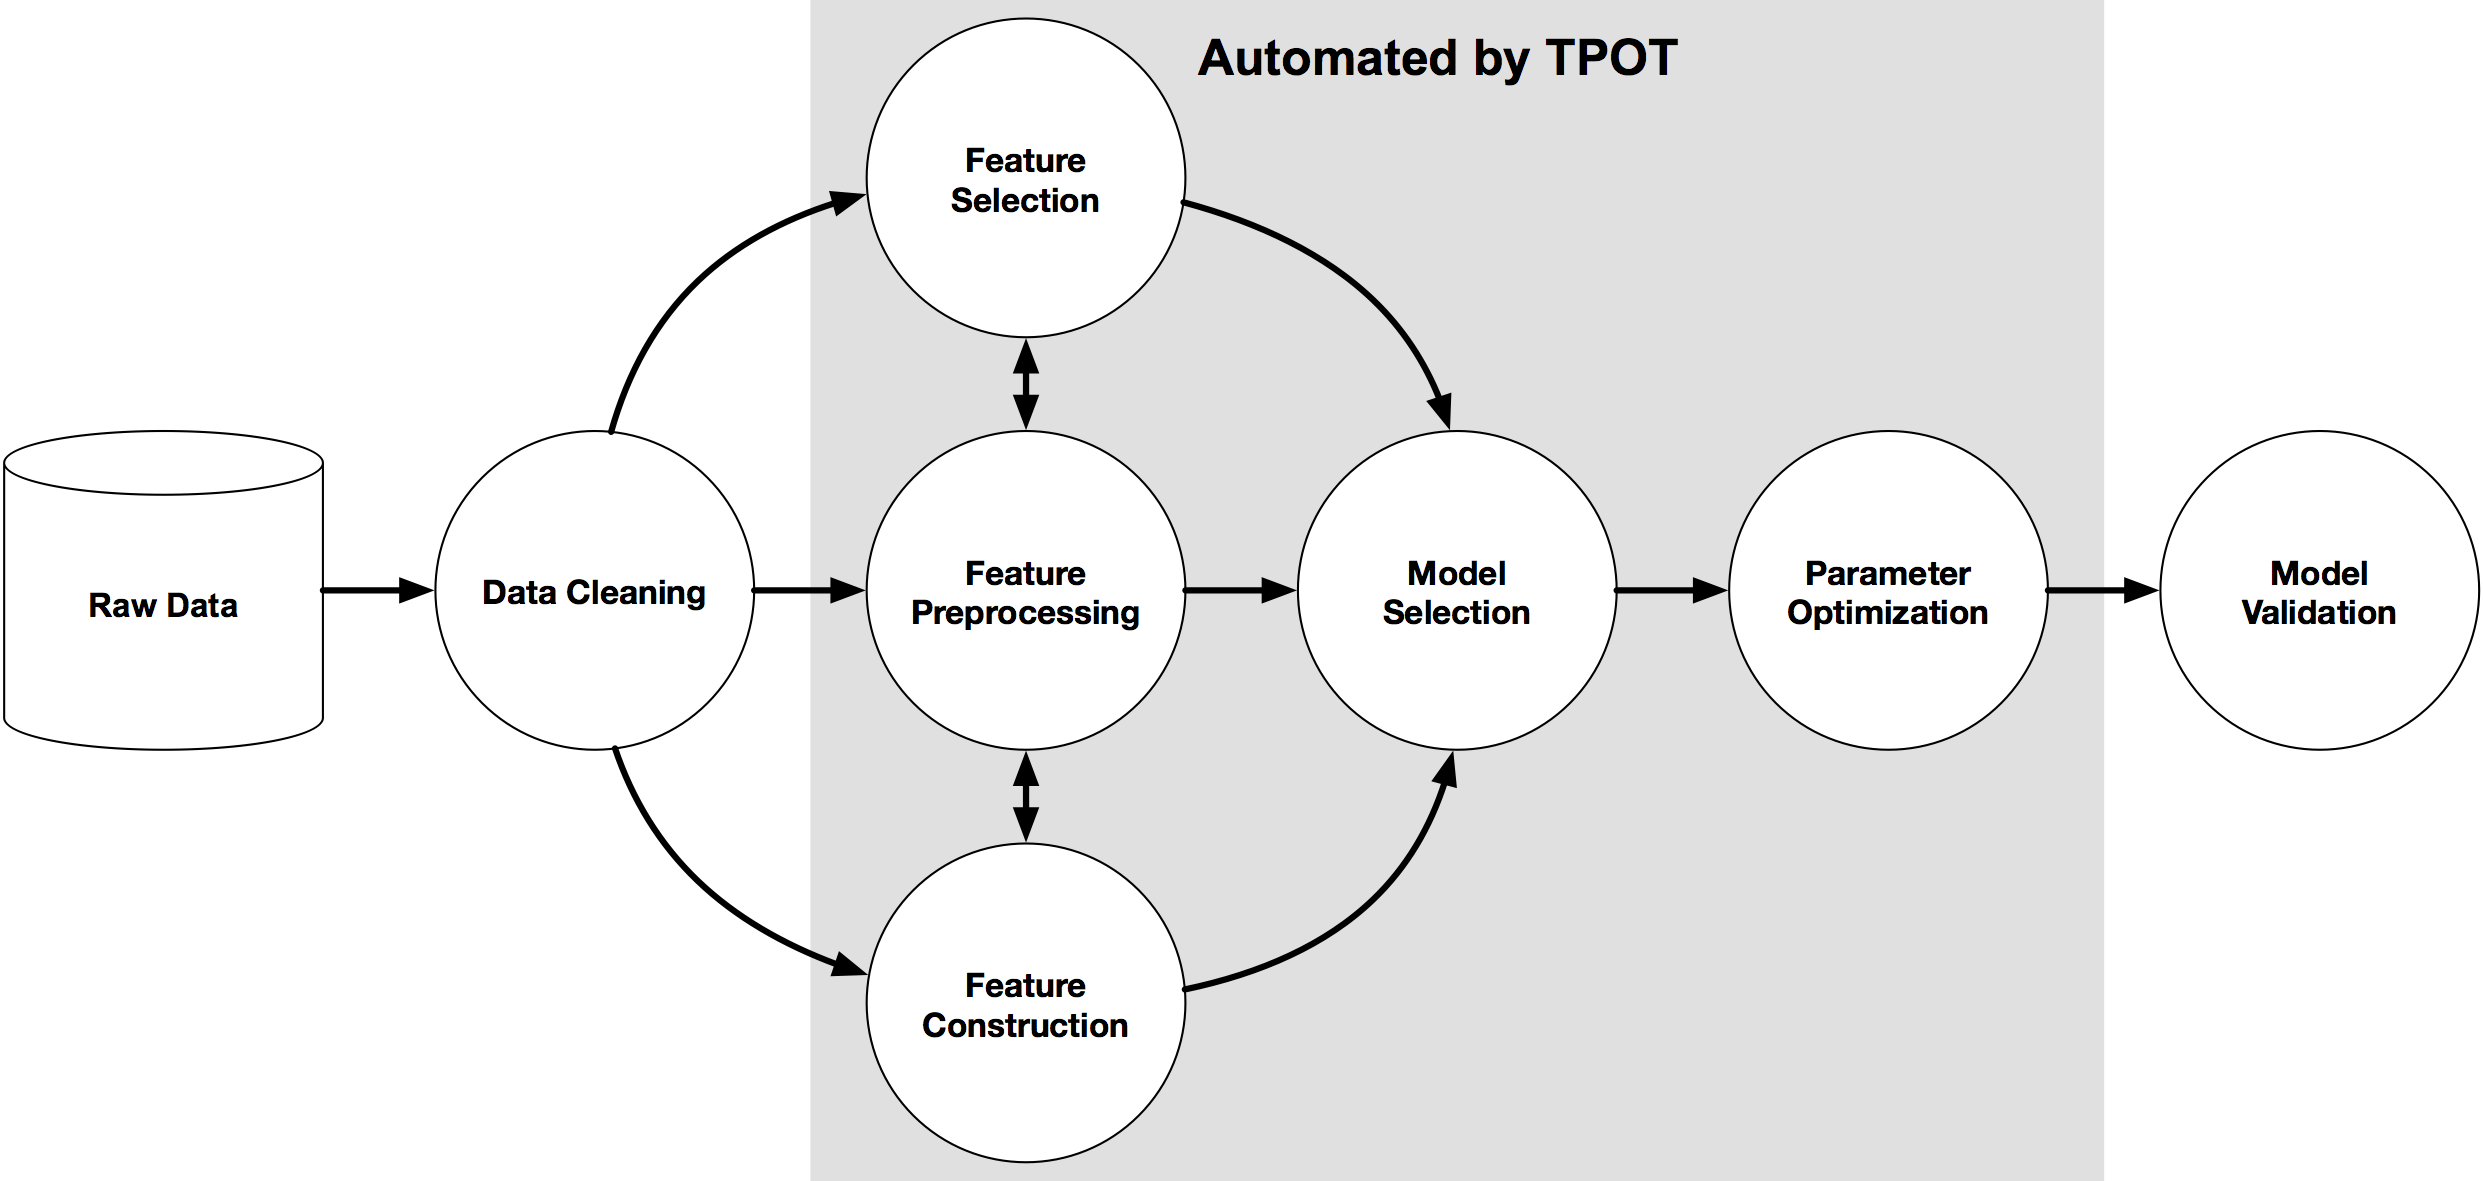
\includegraphics[height=5cm]{images/tpot-ml-pipeline}
 \caption{TPOT 管道流程示意图}
 \label{fig:tpot}
\end{figure}

使用默认参数,TPOT 优化器会创建 100 个流水线,每个流水线演化 100 代,得出这 1 万个流水线的评分。使用十折交叉验证,这意味着将有 10 万次训练要跑!训练过程是非常缓慢的,需要消耗极大的计算资源。从图\ref{fig:360min}中可以看到,即使训练时间设定为6小时,在谷歌云 30GB 的 VM上跑程序,6小时之内也只能演化3代,也就是说这么长的时间内, TPOT 也是非常有可能没有搜寻到最佳流水线的。返回的结果,只能是当前最优流水线。需要注意的是 TPOT 的结果,相同参数下,多次运行的结果也可能不一样。
\begin{figure}[ht]
 \centering
 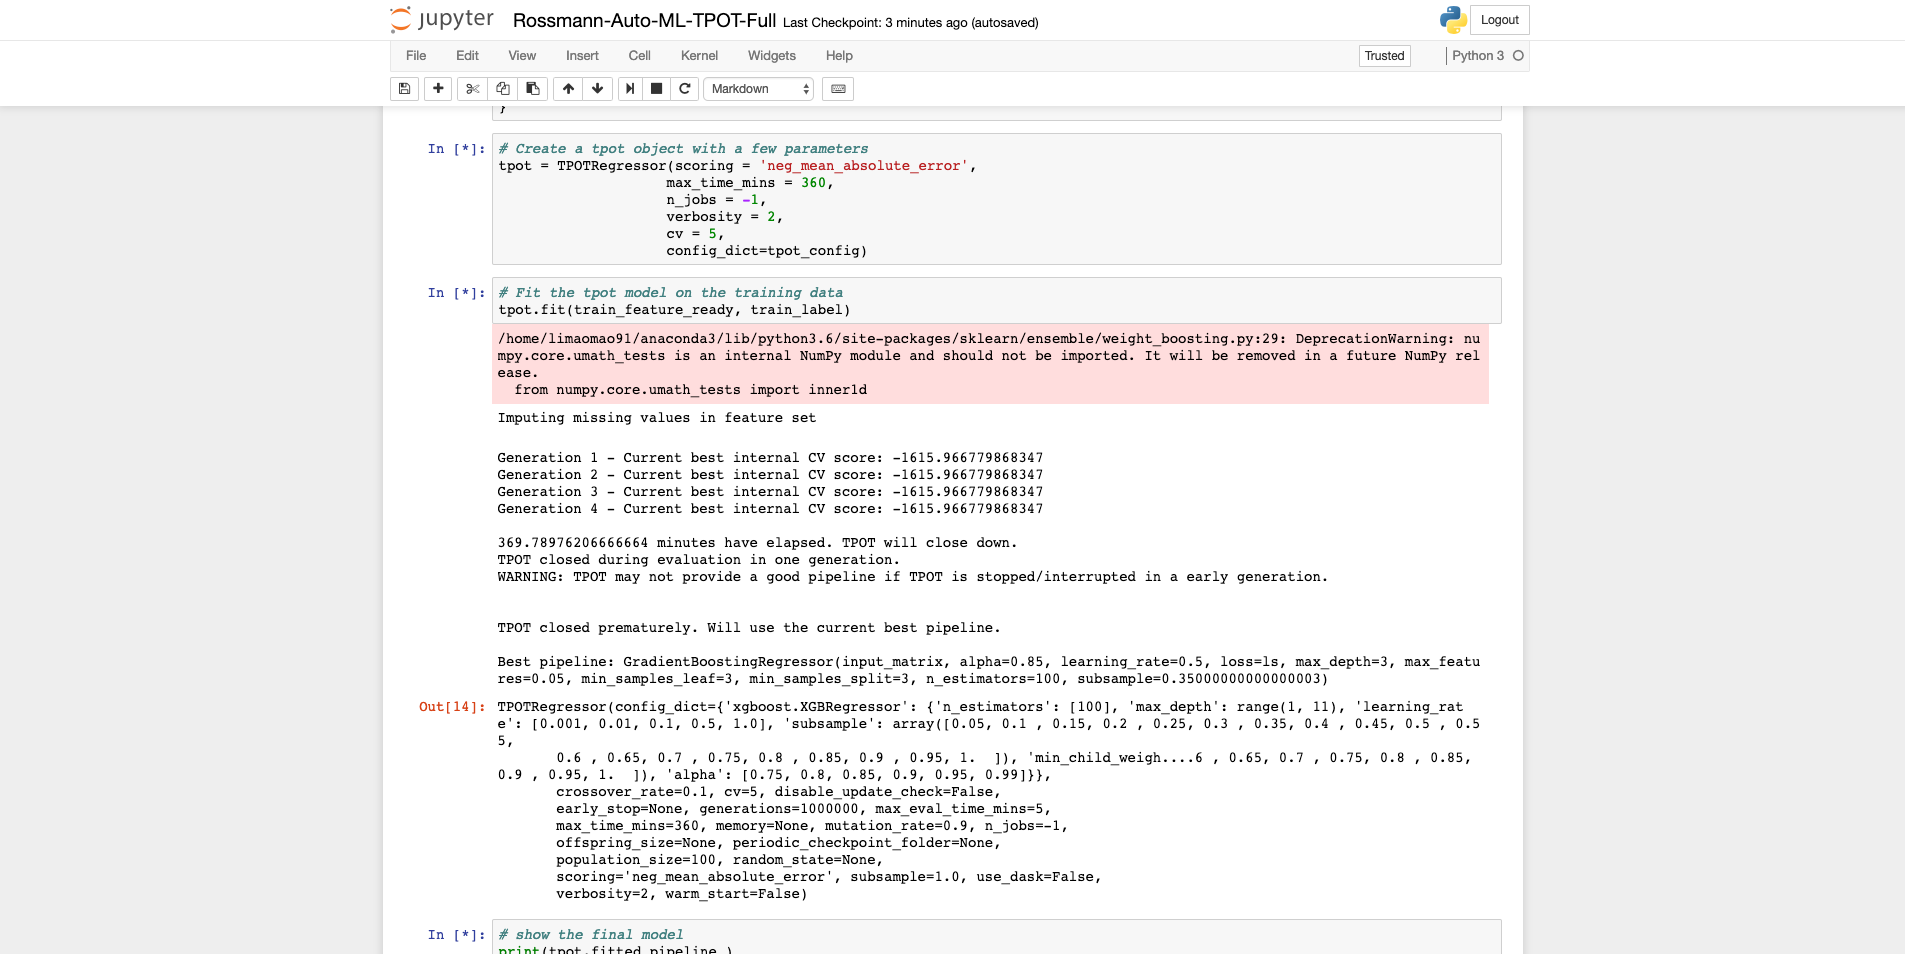
\includegraphics[height=5cm]{images/360min}
 \caption{TPOT 搜索最佳 pipeline 过程}
 \label{fig:360min}
\end{figure}

本项目中,为了丰富自己的技能,同时检验 TPOT 的效果,我们也用了 TPOT 来自动化 Pipeline,寻找选择 model. 现在为止选到的最优化模型为 Gradient Descent Boost, 对应的项目代码,\href{https://github.com/lidatou1991/udacity_final_rossmann/blob/master/Rossmann-Auto-ML-TPOT-Full.ipynb}{TPOT}。需要注意的是,在使用 TPOT 的时候,我们默认 TPOT 是可以帮助我们完成特征工程以及优化调参的,也就是说,我们不需要做任何提前处理。在没有调参、没有增加特征的情况下,图\ref{fig:tpot-gd}目显示前在 leaderboard 上的得分为 0.168。应该说是不尽如人意的,比 Adaboost 的得分都低很多。在完成 xgboost 模型后,再回过头来对比 TPOT 搜索到的 gradient descent 模型参数,我们可以发现,在 learning rate 上值变大以及max depth 等参数上值偏小,都可能是导致TPOT 模型的不够精确,错过最佳参数组合的原因。
\begin{figure}[ht]
 \centering
 
\includegraphics[height=1.5cm,width=\textwidth]{images/tpot-gd-168}
 \caption{Gradient Descent 模型在 leaderboard 得分}
 \label{fig:tpot-gd}
\end{figure}

为了能够在本地机器上方便调试 TPOT,可以在 TPOT 的 config-dic 参数中设置 light mode. 也就是,TPOT 会在简单的流水线中进行搜索。设置之后,TPOT 返回的最佳模型的 KNearestNeighbor Regressor,出乎意料的是,图\ref{fig:knn}得分居然可以到0.14,也就是比复杂的 gradient descent 模型排名还靠前很多。这也说明模型并不一定要越复杂越好。

\begin{figure}[ht]
 \centering
 
\includegraphics[height=1.5cm,width=\textwidth]{images/knn}
 \caption{Knearest Neighbor 模型在 leaderboard 得分}
 \label{fig:knn}
\end{figure}

\section{xgboost 模型}
xgboost 的全称是 (eXtrem Gradient Boost), 首先和 Adaboost 一样,本质上都是决策树 (Decision Tree) 模型,同时是一种 ensemble method,也就是合成算法。图\ref{fig:twocart}是来至于 Xgboost官网的示意图,每个叶节点输出权重值 Weight.

\begin{figure}[ht]
 \centering
 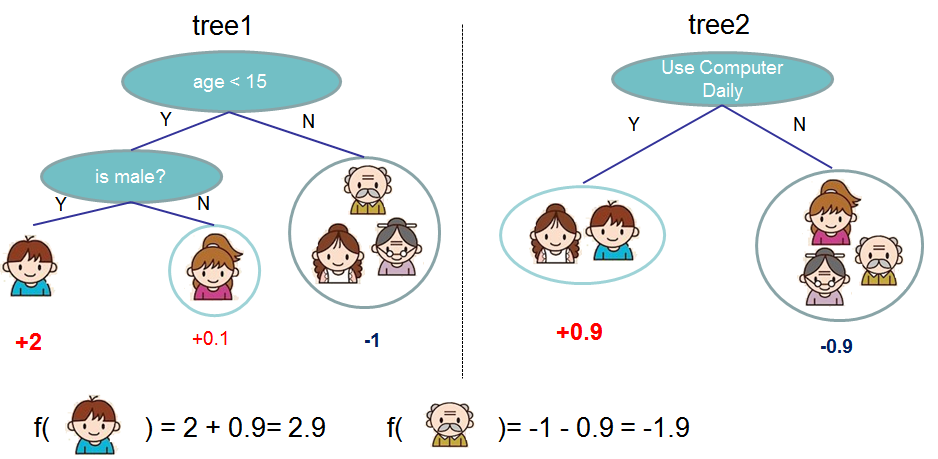
\includegraphics[height=5cm,width=\textwidth]{images/twocart}
 \caption{xgboost 决策树示意图}
 \label{fig:twocart}
\end{figure}

但是,bagging 与 boosting 的合成方式是有本质差别的,如图\ref{fig:ensemble}所示。

\begin{figure}[ht]
 \centering
 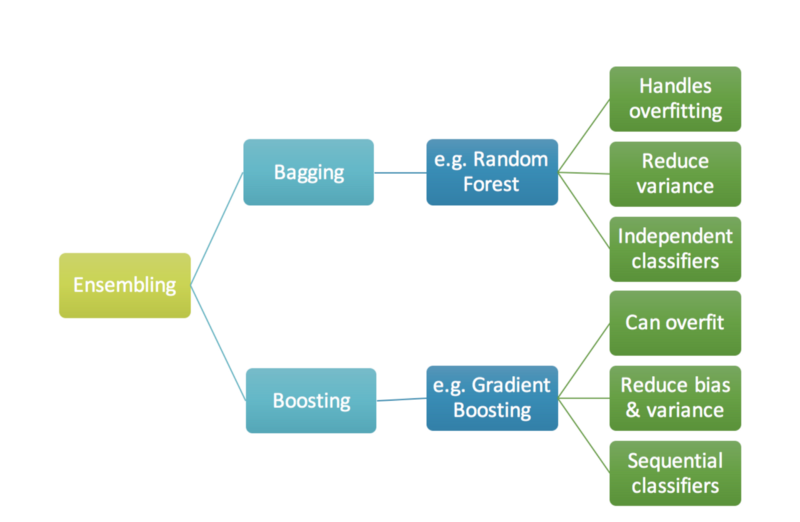
\includegraphics[height=5cm,width=\textwidth]{images/ensemble}
 \caption{Ensemble 算法}
 \label{fig:ensemble}
\end{figure}




虽然都是 ensemble 算法,但是,与 Adaboost 优化提升方式不同的是,Adaboost 采用 Adaptive 的方式提升模型准确度,每次改变的是错误数据的权重。而对于 xgboost,其是在前一次模型训练后的 residual error 上再多次训练模型,然后累加到之前的模型上。下图\ref{fig:residual}展示的是 xgboost 模型的提升过程。

\begin{figure}[ht]
 \centering
 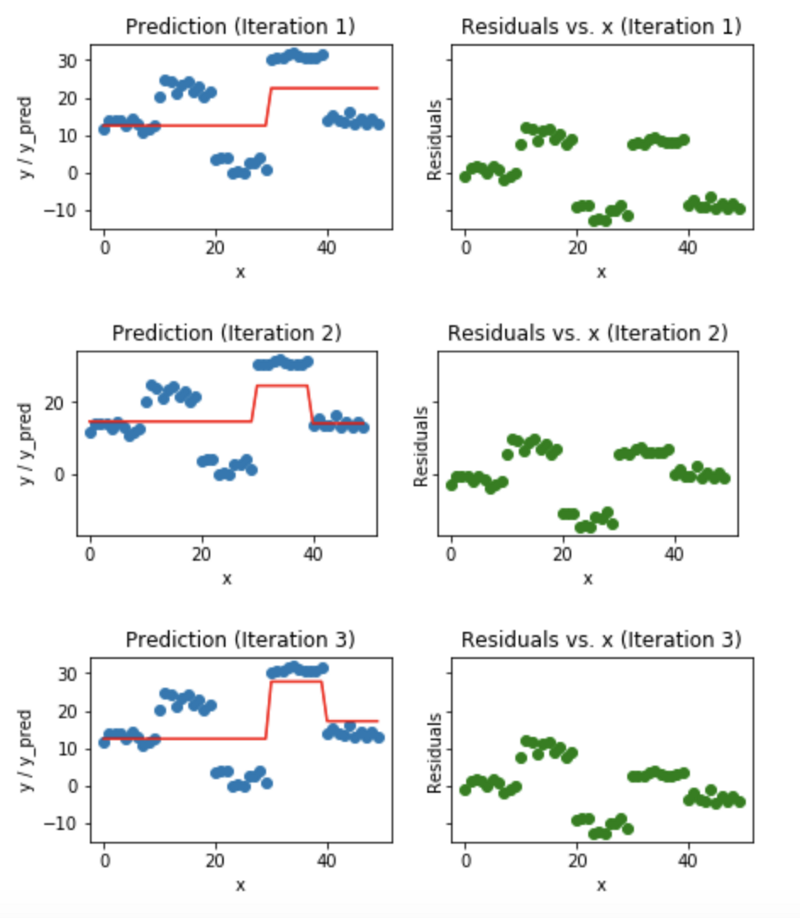
\includegraphics[height=5cm,width=\textwidth]{images/residual}
 \caption{xgboost 通过 minimize residual error 提升模型}
 \label{fig:residual}
\end{figure}



xgboost 是 Gradient Boosting Machine 的一个 C++ 实现,最大的特点在于它能够自动利用 CPU 的多线程进行并行,同时在算法上加以改进提高了精度。为了方便使用,作者陈天奇将 xgboost 封装成了 Python 库。传统 GBDT 在优化时只用到一阶导数信息,xgboost 则对代价函数进行了二阶泰勒展开,同时用到了一阶和二阶导数。xgboost 在代价函数中加入了正则项,用于控制模型的复杂度,学习出来的模型更加简单,防止过拟合。xgboost 在进行完一次迭代后,会将叶子节点的权重乘上缩减(shrinkage)系数,主要是为了削弱每棵树的影响,让后面有更大的学习空间。

\subsection{xgboost 模型结果}
图\ref{fig:best-score}是模型的最佳得分0.11888,基本达到前百分之十的要求。
\begin{figure}[ht]
 \centering
 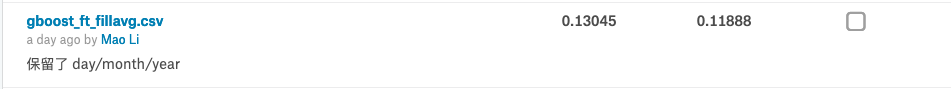
\includegraphics[height=1.5cm,width=\textwidth]{images/best-score}
 \caption{xgboost 最佳得分0.11888}
 \label{fig:best-score}
\end{figure}
此时的 xgboost 的参数如下:
\begin{itemize}
    \item "objective": "reg:linear",
          "booster" : "gbtree",
          "eta": 0.01,
          "max depth": 10,
          "min child weight": 6,
          "subsample": 0.9,
          "colsample bytree": 0.6,
          "silent": 1,
          "seed": 1301
    \item num boost round = 5000
    \item early stopping rounds = 100
\end{itemize}
\subsection{Feature importance}
参考其他公开的方法,绘制出各个特征之间的相对 importance,如图\ref{fig:importance ratio}所示。可以看到排名第一的 feature 是竞争者的距离- competition distance! 这个结果是十分出人意料的,万万没有想到这个特征比商店的平均顾客数或者平均销量还重要。这个结果本身也很难解释,因而决定继续挖掘。

\begin{figure}[ht]
 \centering
 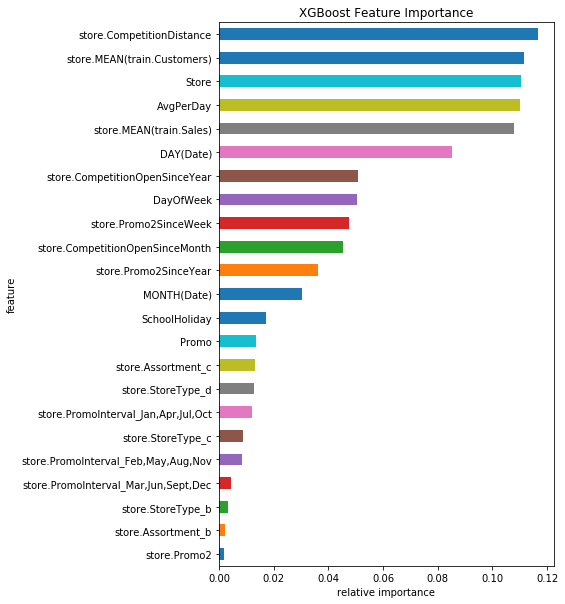
\includegraphics[height=5cm,width=\textwidth]{images/importance}
 \caption{各个特征之间的相对 importance}
 \label{fig:importance ratio}
\end{figure}

查阅了很多资料后发现,xgboost 本身是自带 plot importance 方法的,但是在\href{https://towardsdatascience.com/interpretable-machine-learning-with-xgboost-9ec80d148d27}{文章}中写到 xgboost 自带的feature importance 其实有三种形式:
\begin{itemize}
    \item Weight. The number of times a feature is used to split the data across all trees.
    \item Cover. The number of times a feature is used to split the data across all trees weighted by the number of training data points that go through those splits.
    \item Gain. The average training loss reduction gained when using a feature for splitting.
\end{itemize}
具体到本项目,对应绘制的不同 importance type 下的 feature importance 如下。可以很明显看到,不同 type 下 各个特征的 importance 大相径庭,说明这三种解释方法没有统一性,或者说各有侧重。
\begin{figure}[ht]
 \centering
 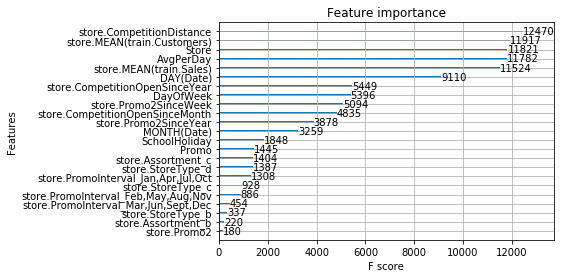
\includegraphics[height=5cm,width=\textwidth]{images/weight}
 \caption{importance type = weight}
 \label{fig:weight}
\end{figure}

\begin{figure}[ht]
 \centering
 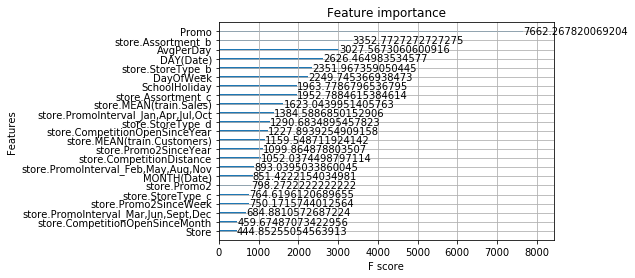
\includegraphics[height=5cm,width=\textwidth]{images/cover}
 \caption{importance type = cover}
 \label{fig:cover}
\end{figure}

\begin{figure}[ht]
 \centering
 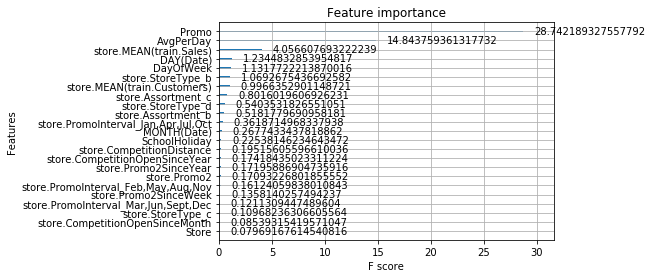
\includegraphics[height=5cm,width=\textwidth]{images/gain}
 \caption{importance type = gain}
 \label{fig:gain}
\end{figure}
简单说,xgboost 的 feature importance plot 实际上是 global importance,对于每个样本在做预测(本项目为回归)的时候的不同 feature 的 importance,显示的其实是做了平均后的结果。也就是说对每个个体的 feature importance 并没有完全反应出来。

同样是来自开发出 xgboost 的华盛顿大学的一个团队,开源了更为统一以及更具有解释性的 xgboost 模型解释库- SHAP.  图\ref{fig:shap-general}展示的是不同 features 对每个预测样本的 feature importance. 每一行的每个点对应一个 sample point. 
\begin{figure}[ht]
 \centering
 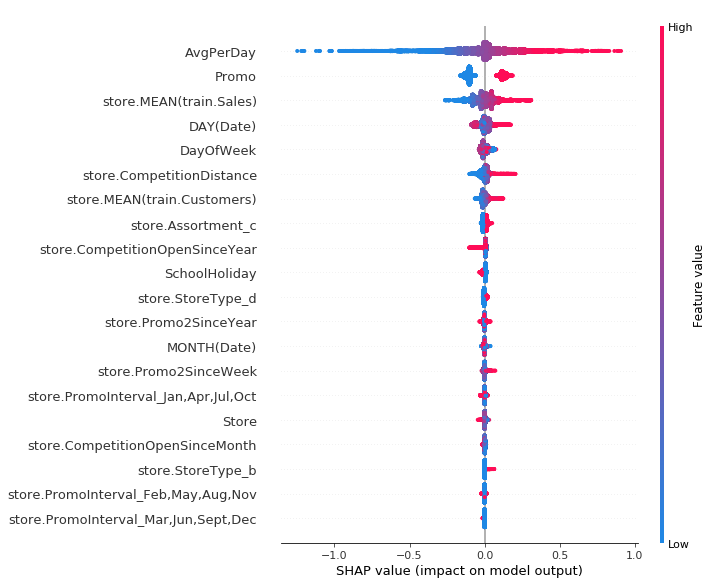
\includegraphics[height=5cm,width=\textwidth]{images/shap-general}
 \caption{SHAP general feature importance}
 \label{fig:shap-general}
\end{figure}
这个时候可以很明显看到,排名前5位的 important feature 分别是:

\begin{itemize}
    \item AvgPerDay: 每周X的X商店的平均销量;
    \item Promo: 是否在促销;
    \item Store.MEAN(train.Sales): X商店平均销量;
    \item DAY(Date):日期
    \item DayOfWeek:星期几
\end{itemize}

这五个特征就相当具有可解释性了,而且和在特征工程时候的预期以及选择基本吻合。SHAP 同时可以研究单个 feature 的影响,或者几个 features 之间的相互影响。图\ref{fig:shap-avg}展示的是两个维度的平均销量的 feature importance. X 轴是星期 X 的平均销量,Y 轴是所有训练集日期的平均销量。很明显 X 值越大 feature importance 值越大。在相同 X值情况下,Y值越大,feature importance 越大,是解释得通的。
\begin{figure}[ht]
 \centering
 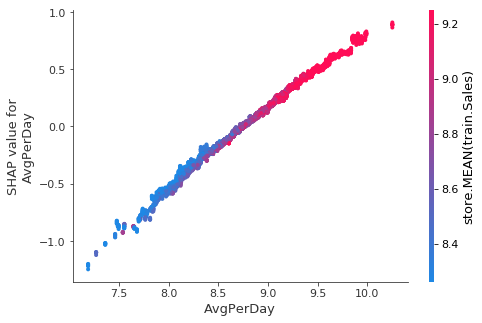
\includegraphics[height=5cm,width=\textwidth]{images/shap-avg}
 \caption{DayOfWeek 平均销量与所有日期平均销量关系}
 \label{fig:shap-avg}
\end{figure}

图\ref{fig:shap-promo}展示的是促销这一特征的 feature  importance,可以明显看到商店在促销的重要性明显大于商店不促销。所有特征之间相互的特征重要性影响如图\ref{fig:shap-interactive}所示,再次需要说明的是,其他的每个点都代表了一个预测样本,因而 SHAP feature importance 是可以细化到每个个体的。
\begin{figure}[ht]
 \centering
 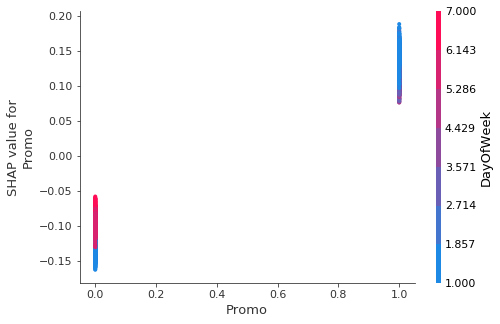
\includegraphics[height=5cm,width=\textwidth]{images/shap-promo}
 \caption{是否促销的 feature importance}
 \label{fig:shap-promo}
\end{figure}

\begin{figure}[ht]
 \centering
 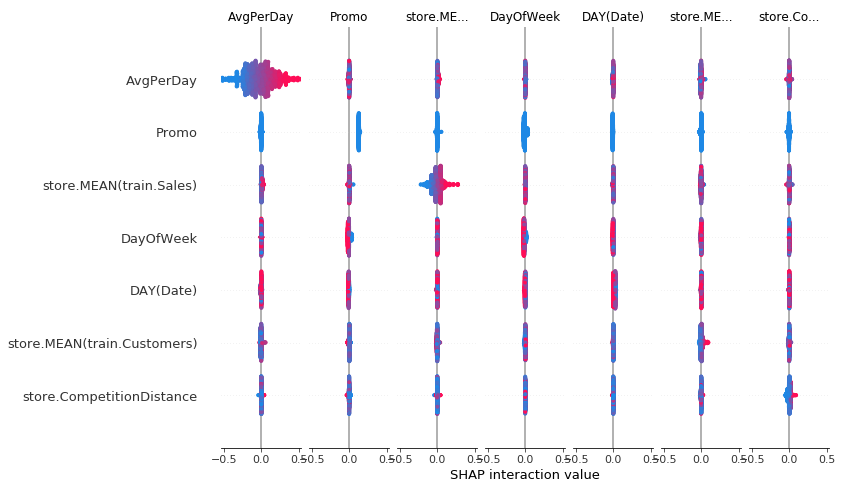
\includegraphics[height=5cm,width=\textwidth]{images/shap-interactive}
 \caption{interactive feature importance}
 \label{fig:shap-interactive}
\end{figure}

xgboost 模型生成的一个决策树的结构如图\ref{fig:hor-tree},其中也可以明显看到每天的平均销量对决策树的结构以及最后的结果有多么重要。
\begin{figure}[ht]
 \centering
 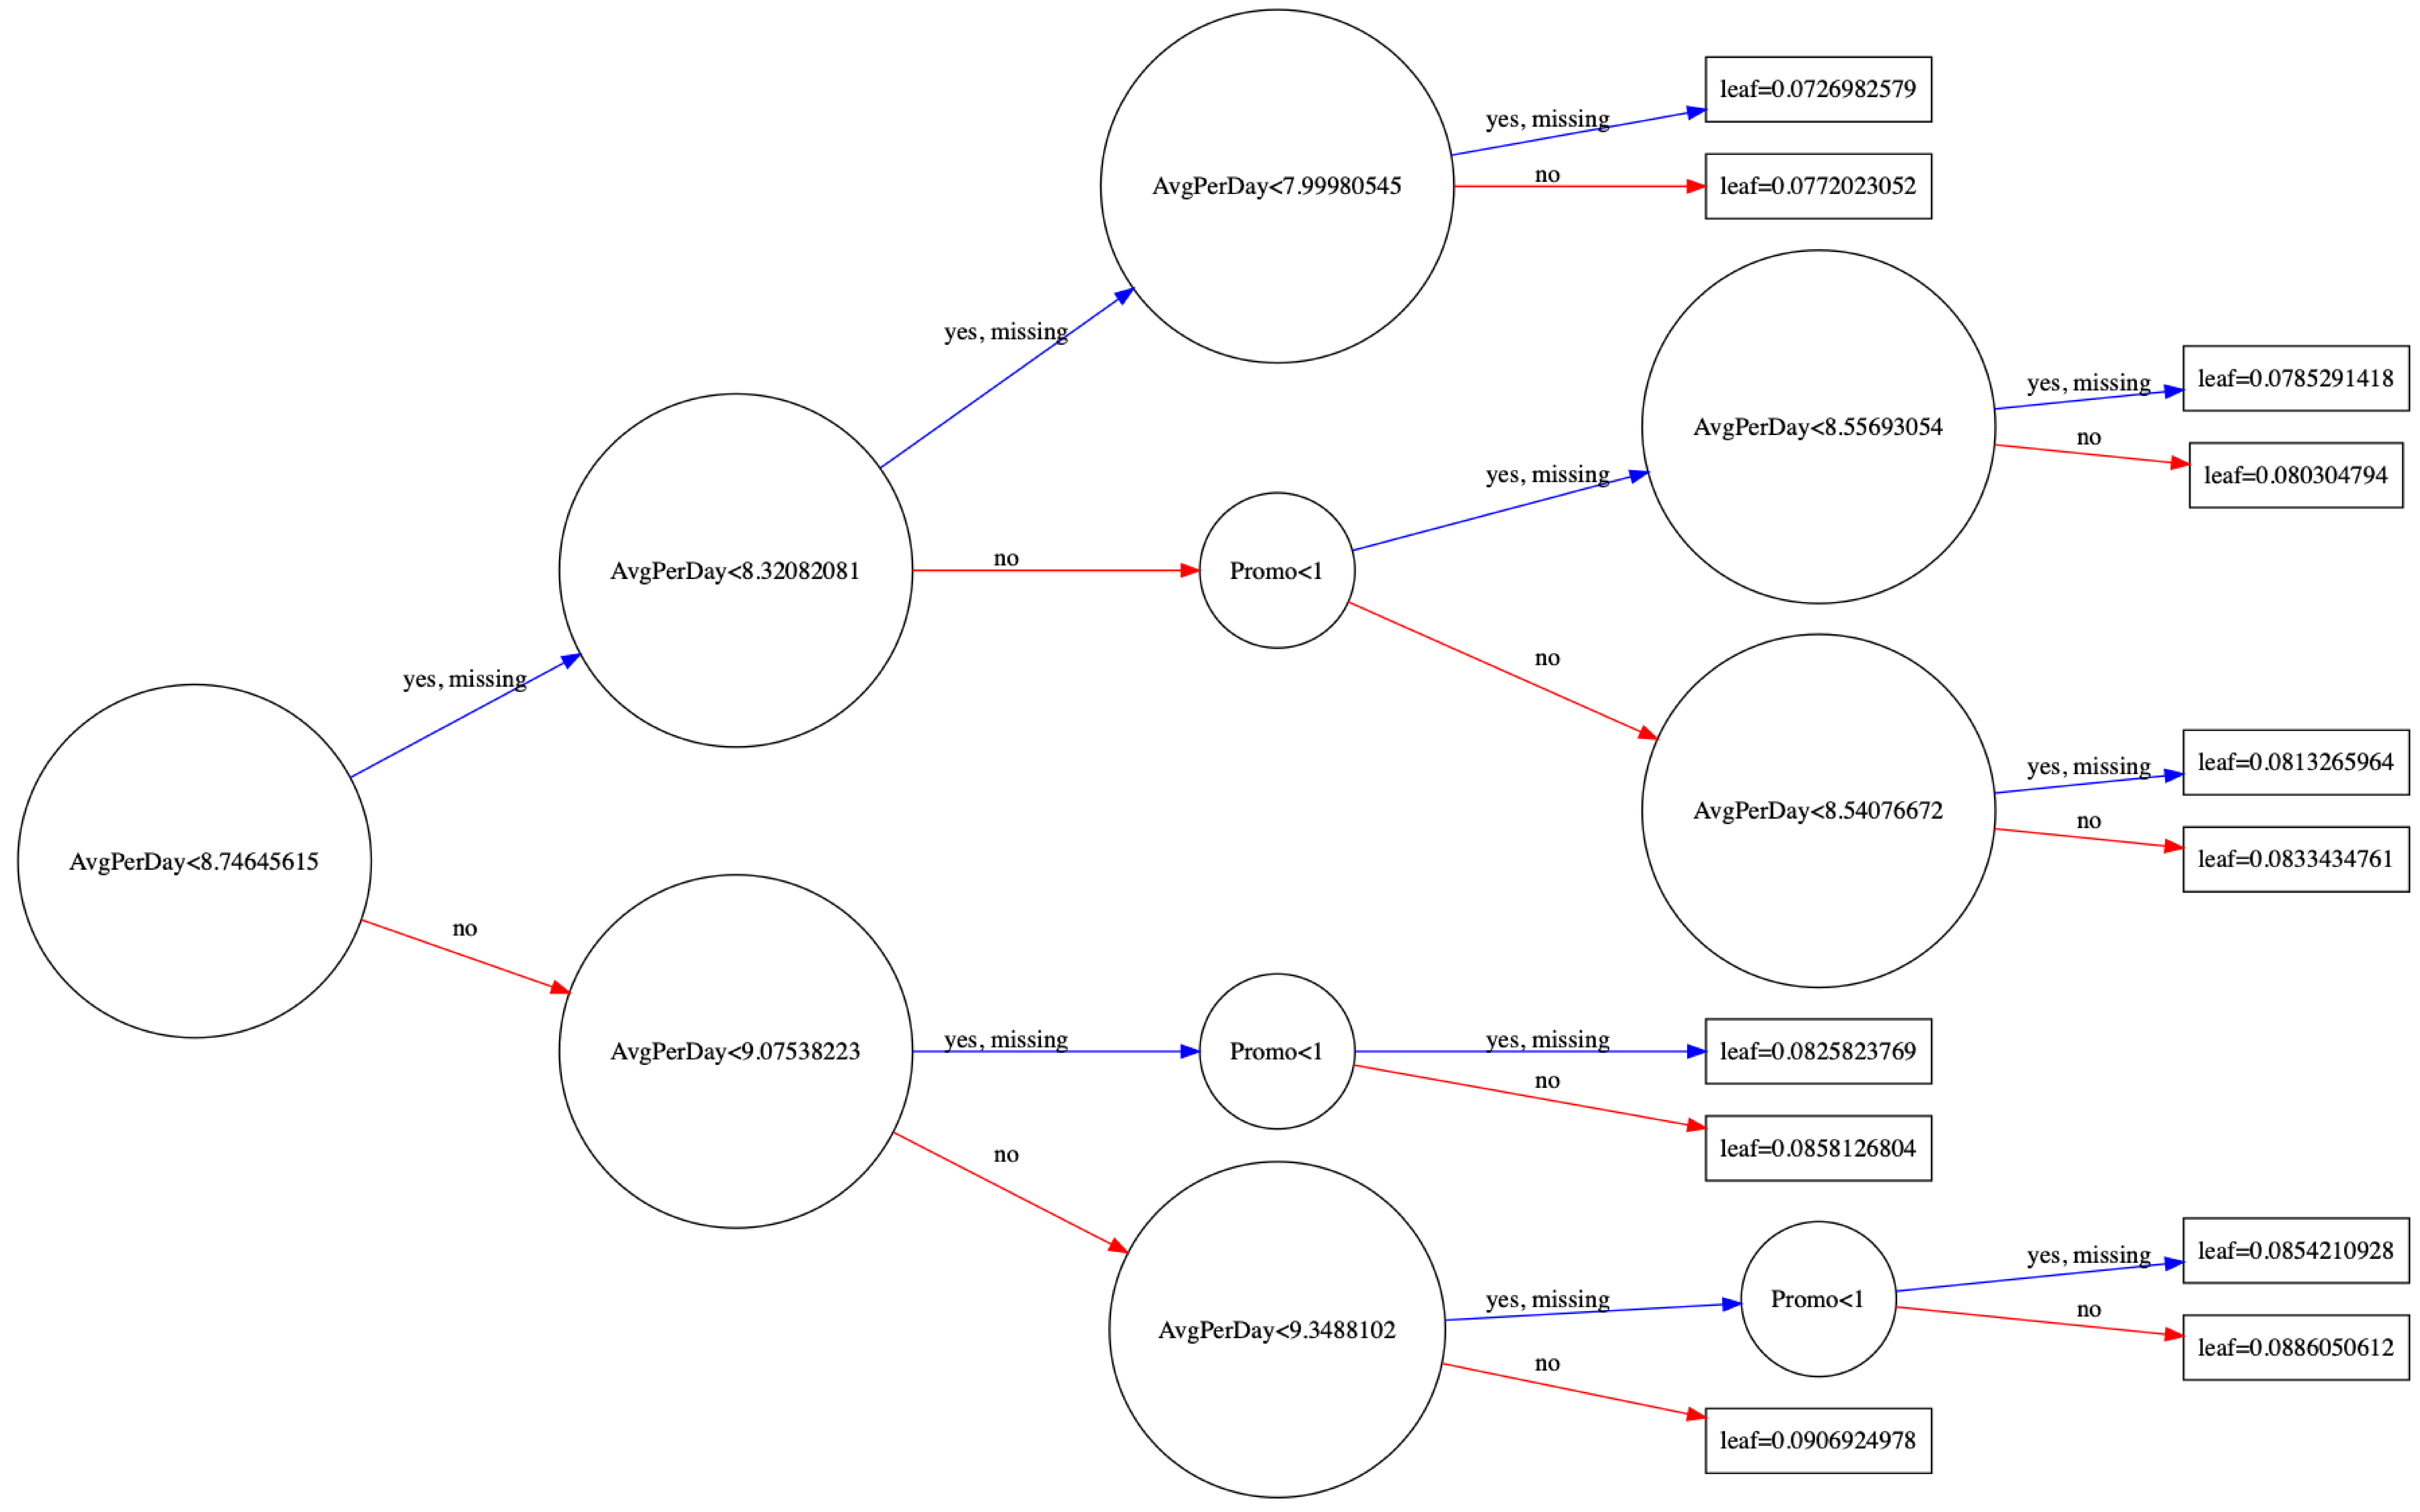
\includegraphics[height=5cm,width=\textwidth]{images/hor-tree}
 \caption{一个决策树模型的结构}
 \label{fig:hor-tree}
\end{figure}
\subsection{模型后处理}
图\ref{fig:store201}和图\ref{fig:ratio201}分别是随机选取的201号商店的预测值与真实值的差异对比。模型后处理的基本思路就是,通过调整权重W,选取出 RMSPE 最小的时候的 W,然后再在预测值中,乘上 W,以期望提高分数。
\begin{figure}[ht]
 \centering
 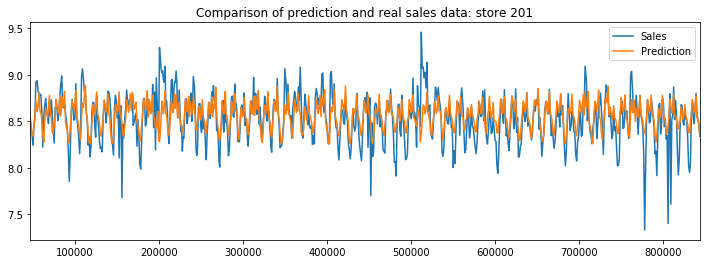
\includegraphics[height=5cm,width=\textwidth]{images/store201}
 \caption{201号商店预测值与hold out 真实值的对比图}
 \label{fig:store201}
\end{figure}

\begin{figure}[ht]
 \centering
 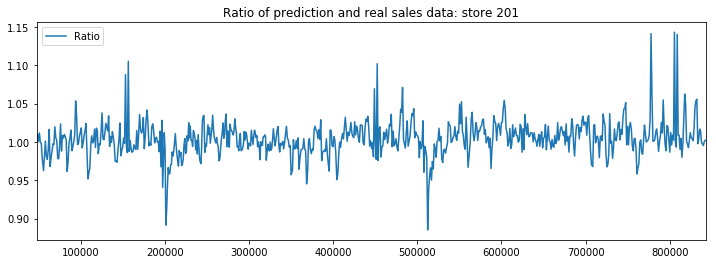
\includegraphics[height=5cm,width=\textwidth]{images/ratio201}
 \caption{201号商店预测值与hold out 真实值的比例图}
 \label{fig:ratio201}
\end{figure}
图\ref{fig:correction-score}是添加修正值前后的得分对比,模型的得分稍有提高,基本达到了前 百分之十。
\begin{figure}[ht]
 \centering
 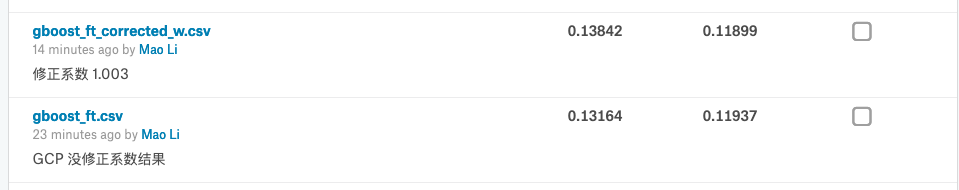
\includegraphics[height=3cm,width=\textwidth]{images/correction-score}
 \caption{修正值添加前后的得分对比}
 \label{fig:correction-score}
\end{figure}
\section{神经网络 Deep Learning Neural Network}\label{keras}
本项目作为 Udacity 机器学习工程师纳米学位课程的毕业项目,除了单单解决问题本身之外,我还希望能够尽可能多地对全部课程的内容进行回顾。此外,本身神经网络模型的预测结果,也完全可能比前面用到的两大类方法所形成的模型更优秀,因而已经有足够多的理由对神经网络模型进行探索。

虽然,神经网络或者深度神经网络模型,现在主流的用处是用于机器视觉(computer vision) 相关问题,而机器视觉问题绝大多数又属于分类问题,例如辨别一张图片是猫还是狗。因而,与本项目的需求之间,也就是做回归预测,还处在一定的差异。但是在查阅网络上的资料后,我发现也是可以用来做回归预测的。

\section{模型对比}

\section{项目后思考}
\subsection{关于项目本身的探索}

\subsection{关于自身的学习所得}
作为非互联网行业从业者以及非计算机科班出身,整体来说通过完整参加 Udacity 机器学习工程师项目,不管是对机器学习理论还是工程代码实现方面都有一定的提高。
\subsection{理论知识}
关于机器学习理论知识,除了观看 Udacity 视频,另外两个最主要的知识来源就是周志华老师的西瓜书——《机器学习》以及互联网上相关博客以及专栏文章。老实讲,西瓜书对于零基础的新手,还算友好:整本书籍有完整的、贯通的讲解方式、入门案例以及数据样例。新手完全可能通过这本书得到一个相对完整的 overview,但是其中的公式推导还是具有一定难度的,毕竟该书还是给大学本科以及研究生专业学习的。但是,这都不影响对基本框架、基本算法的基础理解。

此外,互联网也是进行自我学习的知识宝库。完成整个课程的断断续续半年之中,也发现了很多很好的资源。例如,\href{https://medium.com/}{medium} 平台上的文章质量就很高。尤其是其中的 TwardsDataScience 专栏等,文章水平很高,通常讲解的问题实用又清晰。在这些平台上也发现了很多牛人,在一直做输出,顺通摸瓜追踪到他们的专栏等,都受益匪浅。例如,供职于 Cortex Intel 的数据科学家 \href{https://medium.com/@williamkoehrsen}{Will Koehrsen} 基本上篇篇都是大作。我很多知识点,在 Udacity 视频以及西瓜书上没了解到的,都是通过他的文章。应用在 Rossmann 本项目中的,就是应用 TPOT 框架,自动化机器学习流程——Automated Machine Learning Pipeline. 可以这样讲,如果不看到 Will 的文章,我基本不可能会在本项目中尝试使用 TPOT 框架。虽然在极短暂的时间内,学习 TPOT 遇到了很多坑,但是自己一个一个去踩过之后,还是受益匪浅的。

\subsection{工程代码}
关于工程代码,体会就更多了。首先,作为 Udacity 本身课程来讲,就是定位于工程师应用,所以工程代码能力势必相当重要。回过头来看,自己代码能力还是很弱,这也导致完成毕业项目花费了非常多的时间,主要有以下几个原因:
\begin{itemize}
\item 写的代码量严重不足。首先从课程来讲,虽然说每个单元最后都有 project,但是其实每个 project 的软件环境、基本框架都是搭建好了的,自己只需要写少量的代码。虽然,这有助于提高效率,但是其实自己从零开始,完成一个项目后才知道,这已经让学生少走了很多弯路,少跳了很多坑。而这种局面的对面就是,debug 能力还严重不足。举例来说,在 Google Cloud Platform 上搭建远程环境,就花了我一晚上的时间,期间遇到很多问题,甚至于 pandas 不同版本的安装后的环境冲突等,都是很耗时间的。加之,本来对 Linux 系统也不太熟悉。
\item 思维欠缺系统性。这应该是和自己专业相关,毕竟没有受过系统的、正规的代码能力培训,写出来的代码很散、很杂,运行起来效率也不高。现阶段,自己还处于只要能够代码不报错,能够跑起来就 ok 的水平。例如,在完成本项目过程中,网上查找资料的时候,发现绝大多数做过本项目的人,都是对特征工程中,提取特征单独写了 .py 文件。反过来看自己,首先肯定是水平就不足,完成没想到这种模块化、函数化的思想,加之 jupyter notebook 环境本身 interactive 的编码环境,自己就写一句调试一句。这种方式,给后来的调试造成了很大的麻烦。例如,特征中需要有很多特征要做 one-hot encoding ,加上 notebook 中变量的值又与代码的执行顺序有关,导致在第一个模型——Decision Tree 中就调试了很久。最后,查找到原因,都是由于这些独热编码特征造成的,一会儿造成训练好的模型数据输入类型不对,一会儿又是在test数据集上无法运行。
\end{itemize}

% -----------------------------------Appendix----------------------------------------

% -----------------------------------REFERENCE----------------------------------------
%\begin{thebibliography}{9}
%\bibitem{Erdos01} P. Erd\H os, \emph{A selection of problems and
%results in combinatorics}, Recent trends in combinatorics (Matrahaza,
%1995), Cambridge Univ. Press, Cambridge, 2001, pp. 1--6.
%\end{thebibliography}
\end{document}

